% !TeX encoding = UTF-8
\documentclass[a4paper]{article}
\usepackage{cmap}
\usepackage[utf8]{inputenc}
\usepackage[T2A]{fontenc}
\usepackage[english,russian]{babel}
\usepackage[left=15mm, top=15mm, right=15mm, bottom=25mm, nohead, nofoot]{geometry}
\usepackage{graphicx}
\usepackage{float}
\usepackage{wrapfig}
\usepackage{tikz}
\usepackage{xcolor}
\usepackage{nicefrac}
\usepackage{cancel}
\usepackage{amsmath,amsfonts,amssymb}
\usepackage{fancybox,fancyhdr}
\usepackage{listings}
\usepackage{subcaption}
\usepackage{mathtools}
\usepackage{hyperref}

% Настройка колонтитулов
\pagestyle{fancy}
\fancyhf{}
\fancyhead[L]{Проектная работа}
\fancyhead[R]{\textit{Сравнение методов регрессии}}
\fancyfoot[C]{\thepage}
\setlength{\headheight}{14.5pt}
\addtolength{\topmargin}{-2.5pt}
\headsep=8mm
\footskip=20mm

% Настройка цветов для гиперссылок
\definecolor{urlcolor}{HTML}{3454D1}
\definecolor{linkcolor}{HTML}{3454D1}
\hypersetup{pdfstartview=FitH, linkcolor=linkcolor, urlcolor=urlcolor, colorlinks=true}

% Настройка стиля для листингов кода
\definecolor{strings}{rgb}{0,0.6,0}
\definecolor{comments}{rgb}{0,0.3,0}
\definecolor{numbers}{rgb}{0.5,0.5,0.5}
\definecolor{keywords}{rgb}{0.09,0.61,0.95}
\definecolor{background}{rgb}{0.97,0.97,0.97}
\lstdefinestyle{codestyle}{
    backgroundcolor=\color{background},
    commentstyle=\color{comments},
    keywordstyle=\color{keywords},
    stringstyle=\color{strings},
    numberstyle=\tiny\color{numbers},
    basicstyle=\ttfamily\footnotesize,
    breakatwhitespace=false,
    breaklines=true,
    captionpos=b,
    inputencoding=utf8,
    keepspaces=true,
    numbers=left,
    numbersep=5pt,
    showspaces=false,
    showstringspaces=false,
    showtabs=false,
    tabsize=2,
    extendedchars=true,
    literate=
    {а}{{\cyra}}1
    {б}{{\cyrb}}1
    {в}{{\cyrv}}1
    {г}{{\cyrg}}1
    {д}{{\cyrd}}1
    {е}{{\cyre}}1
    {ж}{{\cyrzh}}1
    {з}{{\cyrz}}1
    {и}{{\cyri}}1
    {й}{{\cyrishrt}}1
    {к}{{\cyrk}}1
    {л}{{\cyrl}}1
    {м}{{\cyrm}}1
    {н}{{\cyrn}}1
    {о}{{\cyro}}1
    {п}{{\cyrp}}1
    {р}{{\cyrr}}1
    {с}{{\cyrs}}1
    {т}{{\cyrt}}1
    {у}{{\cyru}}1
    {ф}{{\cyrf}}1
    {х}{{\cyrh}}1
    {ц}{{\cyrc}}1
    {ч}{{\cyrch}}1
    {ш}{{\cyrsh}}1
    {щ}{{\cyrshch}}1
    {ъ}{{\cyrhrdsn}}1
    {ы}{{\cyrery}}1
    {ь}{{\cyrsftsn}}1
    {э}{{\cyrerev}}1
    {ю}{{\cyryu}}1
    {я}{{\cyrya}}1
    {А}{{\CYRA}}1
    {Б}{{\CYRB}}1
    {В}{{\CYRV}}1
    {Г}{{\CYRG}}1
    {Д}{{\CYRD}}1
    {Е}{{\CYRE}}1
    {Ж}{{\CYRZH}}1
    {З}{{\CYRZ}}1
    {И}{{\CYRI}}1
    {Й}{{\CYRISHRT}}1
    {К}{{\CYRK}}1
    {Л}{{\CYRL}}1
    {М}{{\CYRM}}1
    {Н}{{\CYRN}}1
    {О}{{\CYRO}}1
    {П}{{\CYRP}}1
    {Р}{{\CYRR}}1
    {С}{{\CYRS}}1
    {Т}{{\CYRT}}1
    {У}{{\CYRU}}1
    {Ф}{{\CYRF}}1
    {Х}{{\CYRH}}1
    {Ц}{{\CYRC}}1
    {Ч}{{\CYRCH}}1
    {Ш}{{\CYRSH}}1
    {Щ}{{\CYRSHCH}}1
    {Ъ}{{\CYRHRDSN}}1
    {Ы}{{\CYRERY}}1
    {Ь}{{\CYRSFTSN}}1
    {Э}{{\CYREREV}}1
    {Ю}{{\CYRYU}}1
    {Я}{{\CYRYA}}1
}

\lstset{style=codestyle}

% Настройка оглавления
\addto\captionsrussian{
  \renewcommand{\contentsname}
    {\centering Содержание}
}

% Дополнительные команды
\newcommand{\e}{\;\text{e}}
\let\oldint\int
\def\int{\oldint\limits}
\newcommand{\at}{\biggr\rvert}

\begin{document}

\begin{titlepage}
    \centering
    \vspace*{1cm}
    
    Министерство науки и высшего образования Российской Федерации
    
    \vspace{0.5cm}
    
    {\large \textbf{ФЕДЕРАЛЬНОЕ ГОСУДАРСТВЕННОЕ}} \\
    {\large \textbf{АВТОНОМНОЕ ОБРАЗОВАТЕЛЬНОЕ}} \\
    {\large \textbf{УЧРЕЖДЕНИЕ ВЫСШЕГО ОБРАЗОВАНИЯ}}
    
    \vspace{0.5cm}
    
    {\large \textbf{«НАЦИОНАЛЬНЫЙ ИССЛЕДОВАТЕЛЬСКИЙ}} \\
    {\large \textbf{УНИВЕРСИТЕТ ИТМО»}}
    
    \vspace{0.5cm}
    
    {\large (УНИВЕРСИТЕТ ИТМО)}
    
    \vspace{1.5cm}
    
    Факультет «Систем управления и робототехники»
    
    \vspace{2cm}
    
    {\large \textbf{ОТЧЕТ}}
    
    \vspace{0.5cm}
    
    {\large \textbf{О ПРОЕКТНОЙ РАБОТЕ}}
    
    \vspace{0.5cm}
    
    По дисциплине «Математическая статистика»
    \vspace{0.5cm}

    {\large \textbf{«Сравнение методов регрессии: линейная регрессия vs. логистическая регрессия vs. метод опорных векторов»}}
    
    \vspace{2cm}
    
    \begin{flushleft}
        Студенты потока Мат Стат 23: \\
        Симонов Илья Александрович, R3236, ИСУ 409560 - аналитика данных, постановка задачи, отчёт, визуализация\\
        Мезенцева Варвара Александровна, R3243, ИСУ 413787 - реализация моделей, программная часть, подготовка данных       
    \end{flushleft}
    
    \vspace{1cm}
    
    \begin{flushleft}
        Преподаватель: \\
        Юрова Татьяна Сергеевна
    \end{flushleft}
    
    \vfill
    
    \centering
    Санкт-Петербург\\
    2025
    
\end{titlepage}

\tableofcontents
\newpage

\section{Постановка задачи}

Целью данной работы является сравнительный анализ трёх методов машинного обучения: линейной регрессии, логистической регрессии и метода опорных векторов (SVM). 

Основные задачи исследования:
\begin{enumerate}
    \item Изучить теоретические основы каждого метода
    \item Реализовать алгоритмы на языке Python с использованием библиотеки scikit-learn
    \item Провести эксперименты на четырёх различных наборах данных
    \item Сравнить производительность методов по различным метрикам качества
    \item Проанализировать области применимости каждого метода
\end{enumerate}

Для исследования используются следующие наборы данных:
\begin{itemize}
    \item \textbf{Insurance} — предсказание стоимости медицинской страховки (регрессия)
    \item \textbf{Wine Quality} — оценка качества вина (регрессия и классификация)
    \item \textbf{Titanic} — предсказание выживаемости пассажиров (классификация)
    \item \textbf{Heart Disease} — диагностика заболеваний сердца (классификация)
\end{itemize}

\section{Краткая теория}

\subsection{Линейная регрессия}

Линейная регрессия — это метод статистического анализа, который моделирует зависимость между зависимой переменной $y$ и одной или несколькими независимыми переменными $x_1, x_2, \ldots, x_n$.

Модель имеет вид:
$$y = \beta_0 + \beta_1 x_1 + \beta_2 x_2 + \ldots + \beta_n x_n + \varepsilon$$

где $\beta_i$ — коэффициенты регрессии, $\varepsilon$ — случайная ошибка.

Коэффициенты находятся методом наименьших квадратов:
$$\min_{\beta} \sum_{i=1}^{m} (y_i - \hat{y}_i)^2$$

\subsection{Логистическая регрессия}

Логистическая регрессия используется для задач бинарной классификации. Она моделирует вероятность принадлежности объекта к определённому классу.

Модель основана на логистической функции:
$$p(y=1|x) = \frac{1}{1 + e^{-(\beta_0 + \beta_1 x_1 + \ldots + \beta_n x_n)}}$$

Коэффициенты находятся методом максимального правдоподобия.

\subsection{Метод опорных векторов (SVM)}

SVM — это метод машинного обучения, который может использоваться как для классификации (SVC), так и для регрессии (SVR).

Основная идея SVM заключается в поиске оптимальной разделяющей гиперплоскости, которая максимизирует отступ между классами.

Для нелинейно разделимых данных используется kernel trick с различными ядрами (RBF, полиномиальное, линейное).

\section{Используемые данные}

\subsection{Insurance Dataset}
\begin{itemize}
    \item \textbf{Размер}: 1338 записей, 7 признаков
    \item \textbf{Цель}: предсказание стоимости медицинской страховки (charges)
    \item \textbf{Признаки}: возраст, пол, BMI, количество детей, курение, регион
    \item \textbf{Тип задачи}: регрессия
\end{itemize}

\subsection{Wine Quality Dataset}
\begin{itemize}
    \item \textbf{Размер}: 6497 записей, 12 признаков
    \item \textbf{Цель}: оценка качества вина (quality, 0-10)
    \item \textbf{Признаки}: кислотность, сахар, pH, алкоголь и др.
    \item \textbf{Тип задачи}: регрессия и классификация (бинаризация по порогу ≥6)
\end{itemize}

\subsection{Titanic Dataset}
\begin{itemize}
    \item \textbf{Размер}: 1309 записей, 11 признаков
    \item \textbf{Цель}: предсказание выживаемости (Survived)
    \item \textbf{Признаки}: класс билета, возраст, пол, количество родственников
    \item \textbf{Тип задачи}: бинарная классификация
\end{itemize}

\subsection{Heart Disease Dataset}
\begin{itemize}
    \item \textbf{Размер}: 1025 записей, 13 признаков
    \item \textbf{Цель}: диагностика заболевания сердца (target)
    \item \textbf{Признаки}: возраст, пол, давление, холестерин и др.
    \item \textbf{Тип задачи}: бинарная классификация
\end{itemize}

\section{Описание моделей и кода}

Проект реализован на языке Python с использованием следующих библиотек:
\begin{itemize}
    \item \texttt{pandas} — работа с данными
    \item \texttt{scikit-learn} — алгоритмы машинного обучения
    \item \texttt{matplotlib, seaborn} — визуализация
    \item \texttt{numpy} — численные вычисления
\end{itemize}

\textbf{Исходный код проекта доступен в GitHub репозитории:}
\url{https://github.com/IlyaKonFetka/MatStatProject.git}

\subsection{Структура проекта}
\begin{itemize}
    \item \texttt{01\_data\_analysis.py} — исследовательский анализ данных
    \item \texttt{02\_preprocessing.py} — предобработка данных
    \item \texttt{03\_linear\_regression.py} — линейная регрессия
    \item \texttt{04\_logistic\_regression.py} — логистическая регрессия
    \item \texttt{05\_svm.py} — метод опорных векторов
    \item \texttt{06\_evaluation.py} — оценка и сравнение моделей
    \item \texttt{main\_pipeline.py} — основной пайплайн
\end{itemize}

\subsection{Предобработка данных}
Для всех датасетов применялись следующие шаги:
\begin{enumerate}
    \item Удаление строк с пропущенными значениями
    \item Разделение на числовые и категориальные признаки
    \item Стандартизация числовых признаков (StandardScaler)
    \item One-Hot кодирование категориальных признаков
    \item Разделение на обучающую и тестовую выборки (80/20)
\end{enumerate}

Предобработка данных является критически важным этапом в машинном обучении. Стандартизация признаков необходима особенно для алгоритмов, чувствительных к масштабу данных, таких как SVM. One-Hot кодирование позволяет работать с категориальными переменными, преобразуя их в числовой формат без создания ложной упорядоченности.

\subsection{Детальное описание алгоритмов}

\subsubsection{Линейная регрессия}
Линейная регрессия является фундаментальным методом статистического анализа. В данной работе использовалась стандартная реализация из scikit-learn, которая применяет метод наименьших квадратов для нахождения оптимальных коэффициентов. 

Преимущества метода:
\begin{itemize}
    \item Простота интерпретации
    \item Быстрота обучения и предсказания
    \item Отсутствие гиперпараметров для настройки
    \item Хорошая работа при линейных зависимостях
\end{itemize}

Недостатки:
\begin{itemize}
    \item Предположение о линейности связи
    \item Чувствительность к выбросам
    \item Проблемы с мультиколлинеарностью
\end{itemize}

\subsubsection{Логистическая регрессия}
Логистическая регрессия адаптирует принципы линейной регрессии для задач классификации. Использовалась реализация с максимальным количеством итераций 1000 для обеспечения сходимости на всех датасетах.

Особенности реализации:
\begin{itemize}
    \item Использование функции потерь логарифмического правдоподобия
    \item Применение сигмоидной функции активации
    \item Регуляризация L2 по умолчанию для предотвращения переобучения
\end{itemize}

\subsubsection{Метод опорных векторов}
SVM реализован в двух вариантах: SVC для классификации и SVR для регрессии. Использовалось RBF-ядро как наиболее универсальное для нелинейных зависимостей.

Ключевые параметры:
\begin{itemize}
    \item Kernel='rbf' — радиальная базисная функция
    \item Probability=True для SVC — получение вероятностных оценок
    \item Параметры C и gamma по умолчанию из scikit-learn
\end{itemize}

\subsection{Метрики оценки}

\subsubsection{Метрики регрессии}
\textbf{RMSE (Root Mean Square Error):}
$$RMSE = \sqrt{\frac{1}{n}\sum_{i=1}^{n}(y_i - \hat{y}_i)^2}$$

RMSE показывает среднеквадратичную ошибку предсказания в тех же единицах, что и целевая переменная. Чем меньше RMSE, тем лучше модель.

\textbf{R² (коэффициент детерминации):}
$$R^2 = 1 - \frac{SS_{res}}{SS_{tot}} = 1 - \frac{\sum_{i=1}^{n}(y_i - \hat{y}_i)^2}{\sum_{i=1}^{n}(y_i - \bar{y})^2}$$

R² показывает долю дисперсии, объясняемую моделью. Значения близкие к 1 указывают на хорошее качество модели.

\subsubsection{Метрики классификации}
\textbf{Accuracy:} доля правильных предсказаний от общего числа предсказаний.

\textbf{F1-score:} гармоническое среднее между точностью (precision) и полнотой (recall):
$$F1 = 2 \cdot \frac{precision \cdot recall}{precision + recall}$$

\textbf{AUC (Area Under Curve):} площадь под ROC-кривой, характеризующая способность модели различать классы.

\section{Графики и визуализации}

\subsection{Корреляционные матрицы датасетов}

Корреляционные матрицы показывают взаимосвязи между числовыми признаками в каждом датасете.

\begin{figure}[H]
\centering
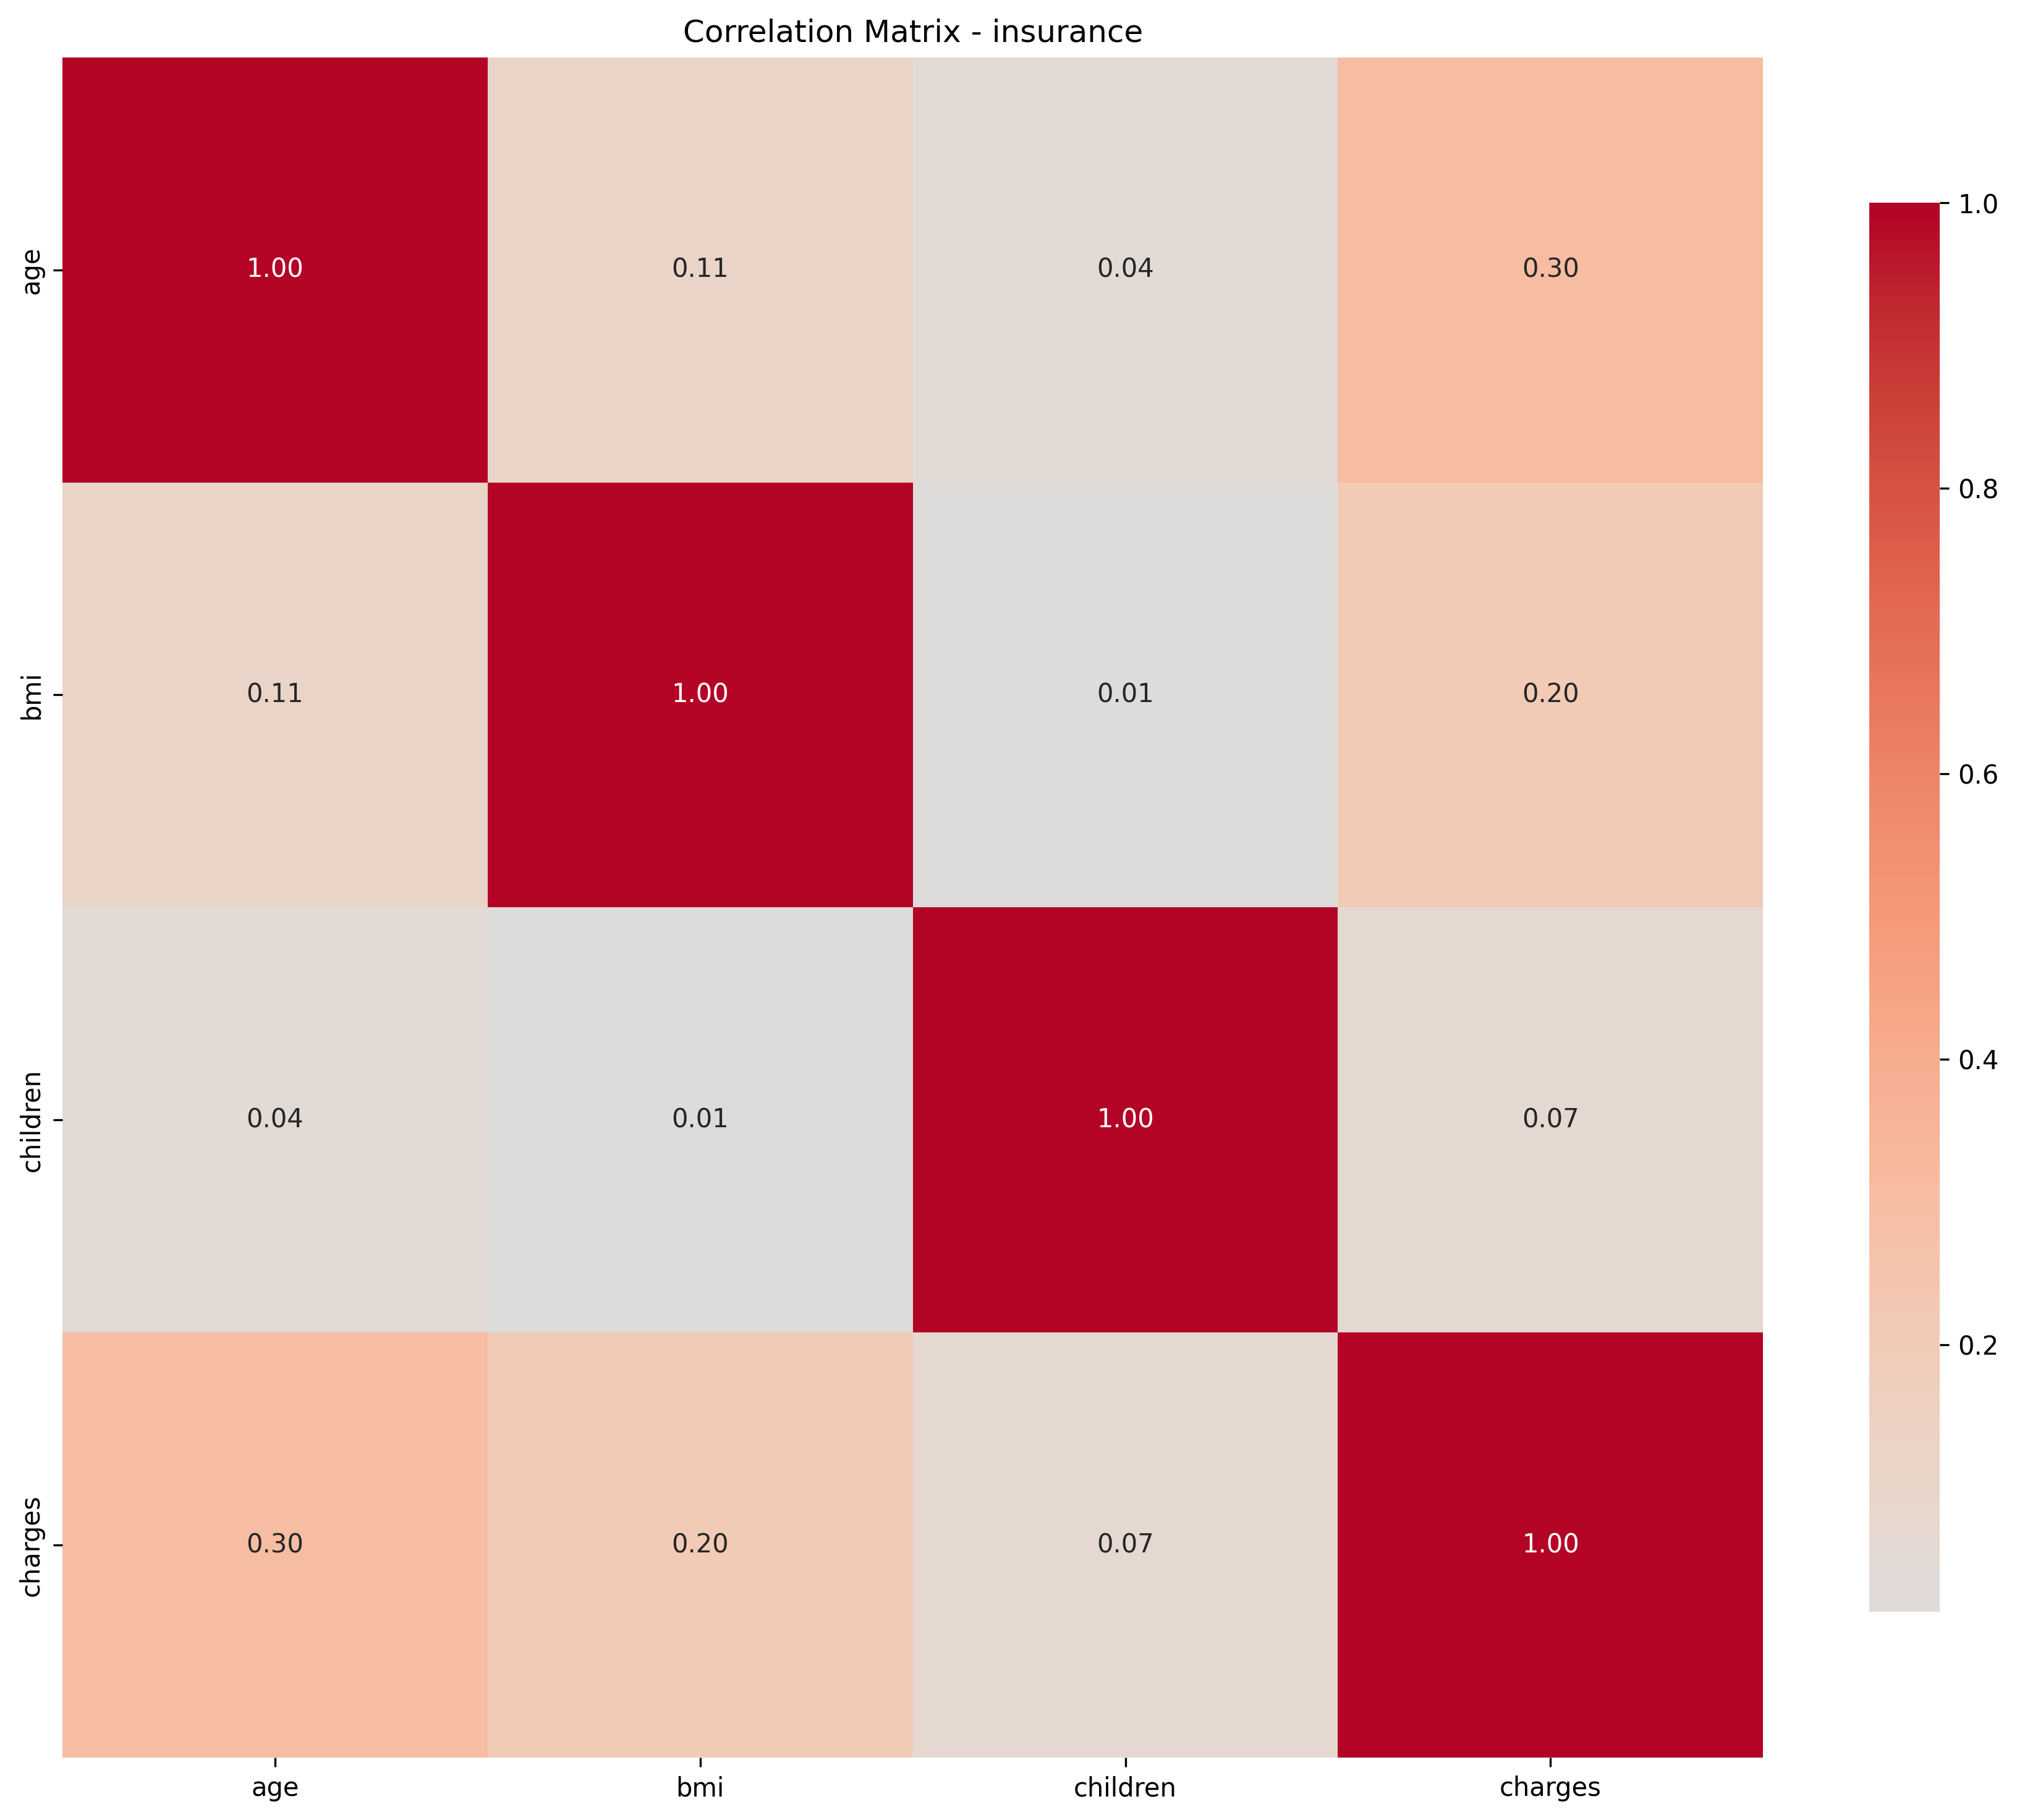
\includegraphics[width=0.7\textwidth]{images/correlation_heatmap_insurance.png}
\caption{Корреляционная матрица — Insurance Dataset}
\end{figure}

\begin{figure}[H]
\centering
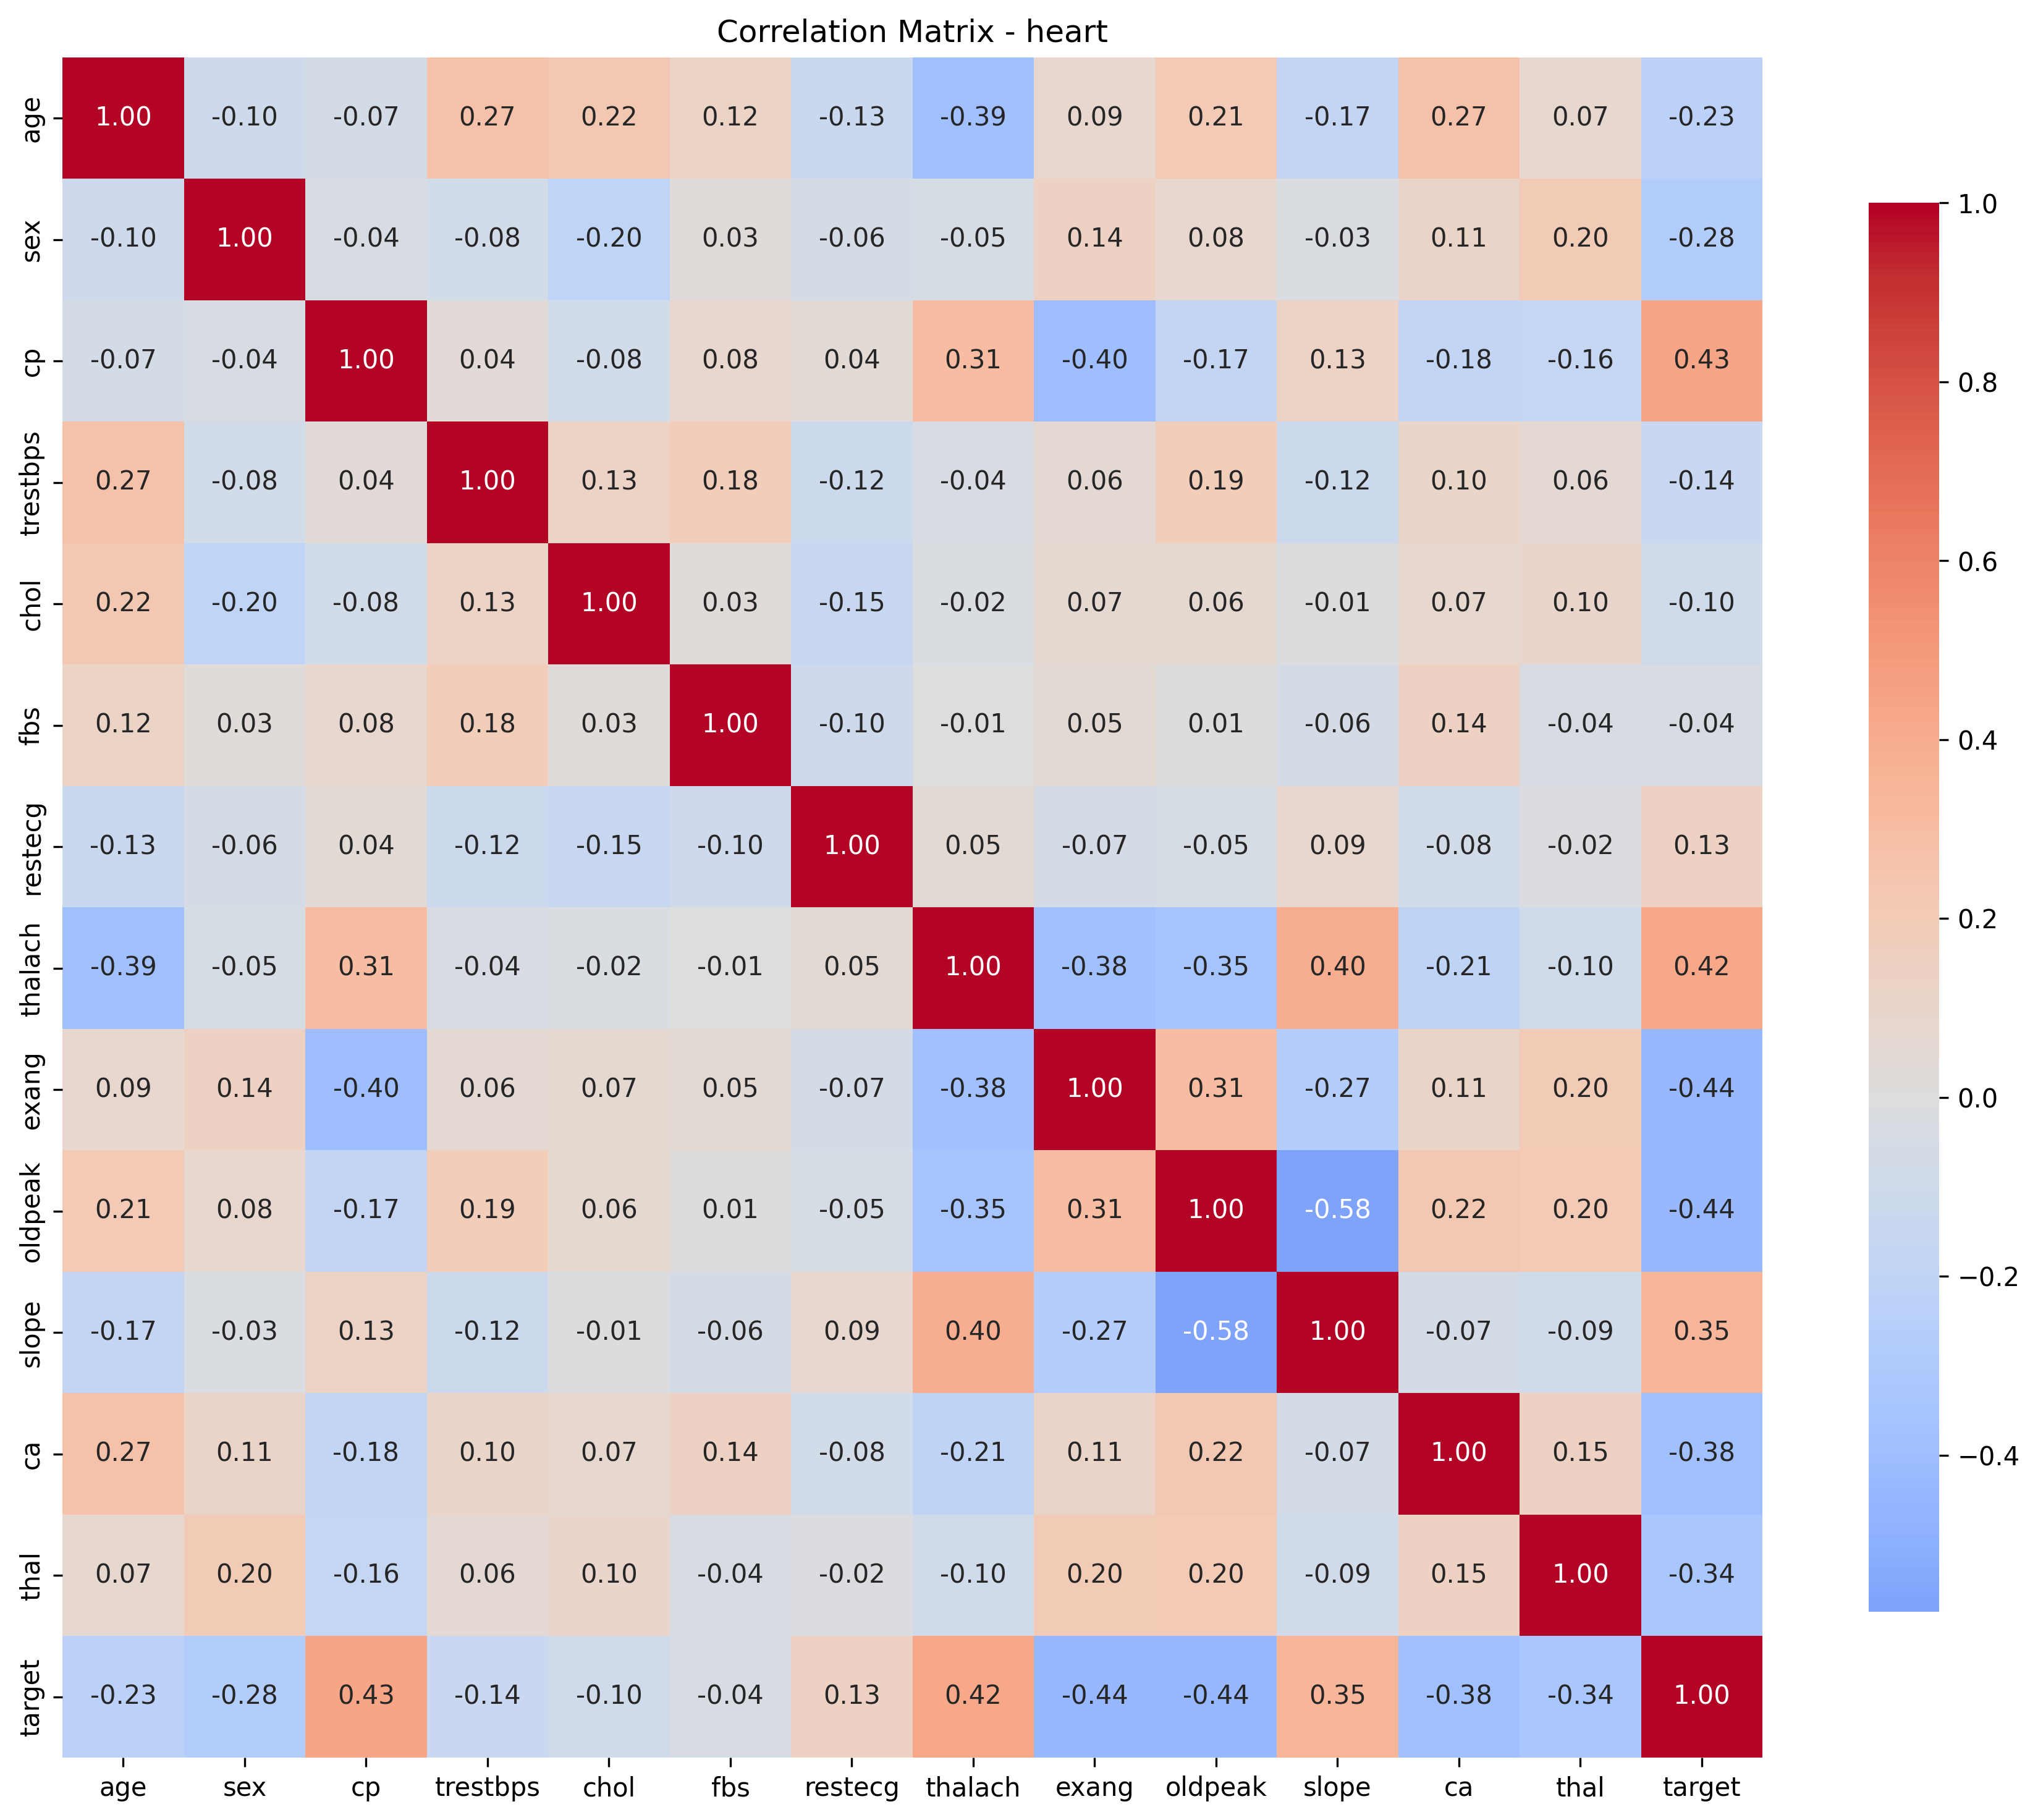
\includegraphics[width=0.7\textwidth]{images/correlation_heatmap_heart.png}
\caption{Корреляционная матрица — Heart Disease Dataset}
\end{figure}

\begin{figure}[H]
\centering
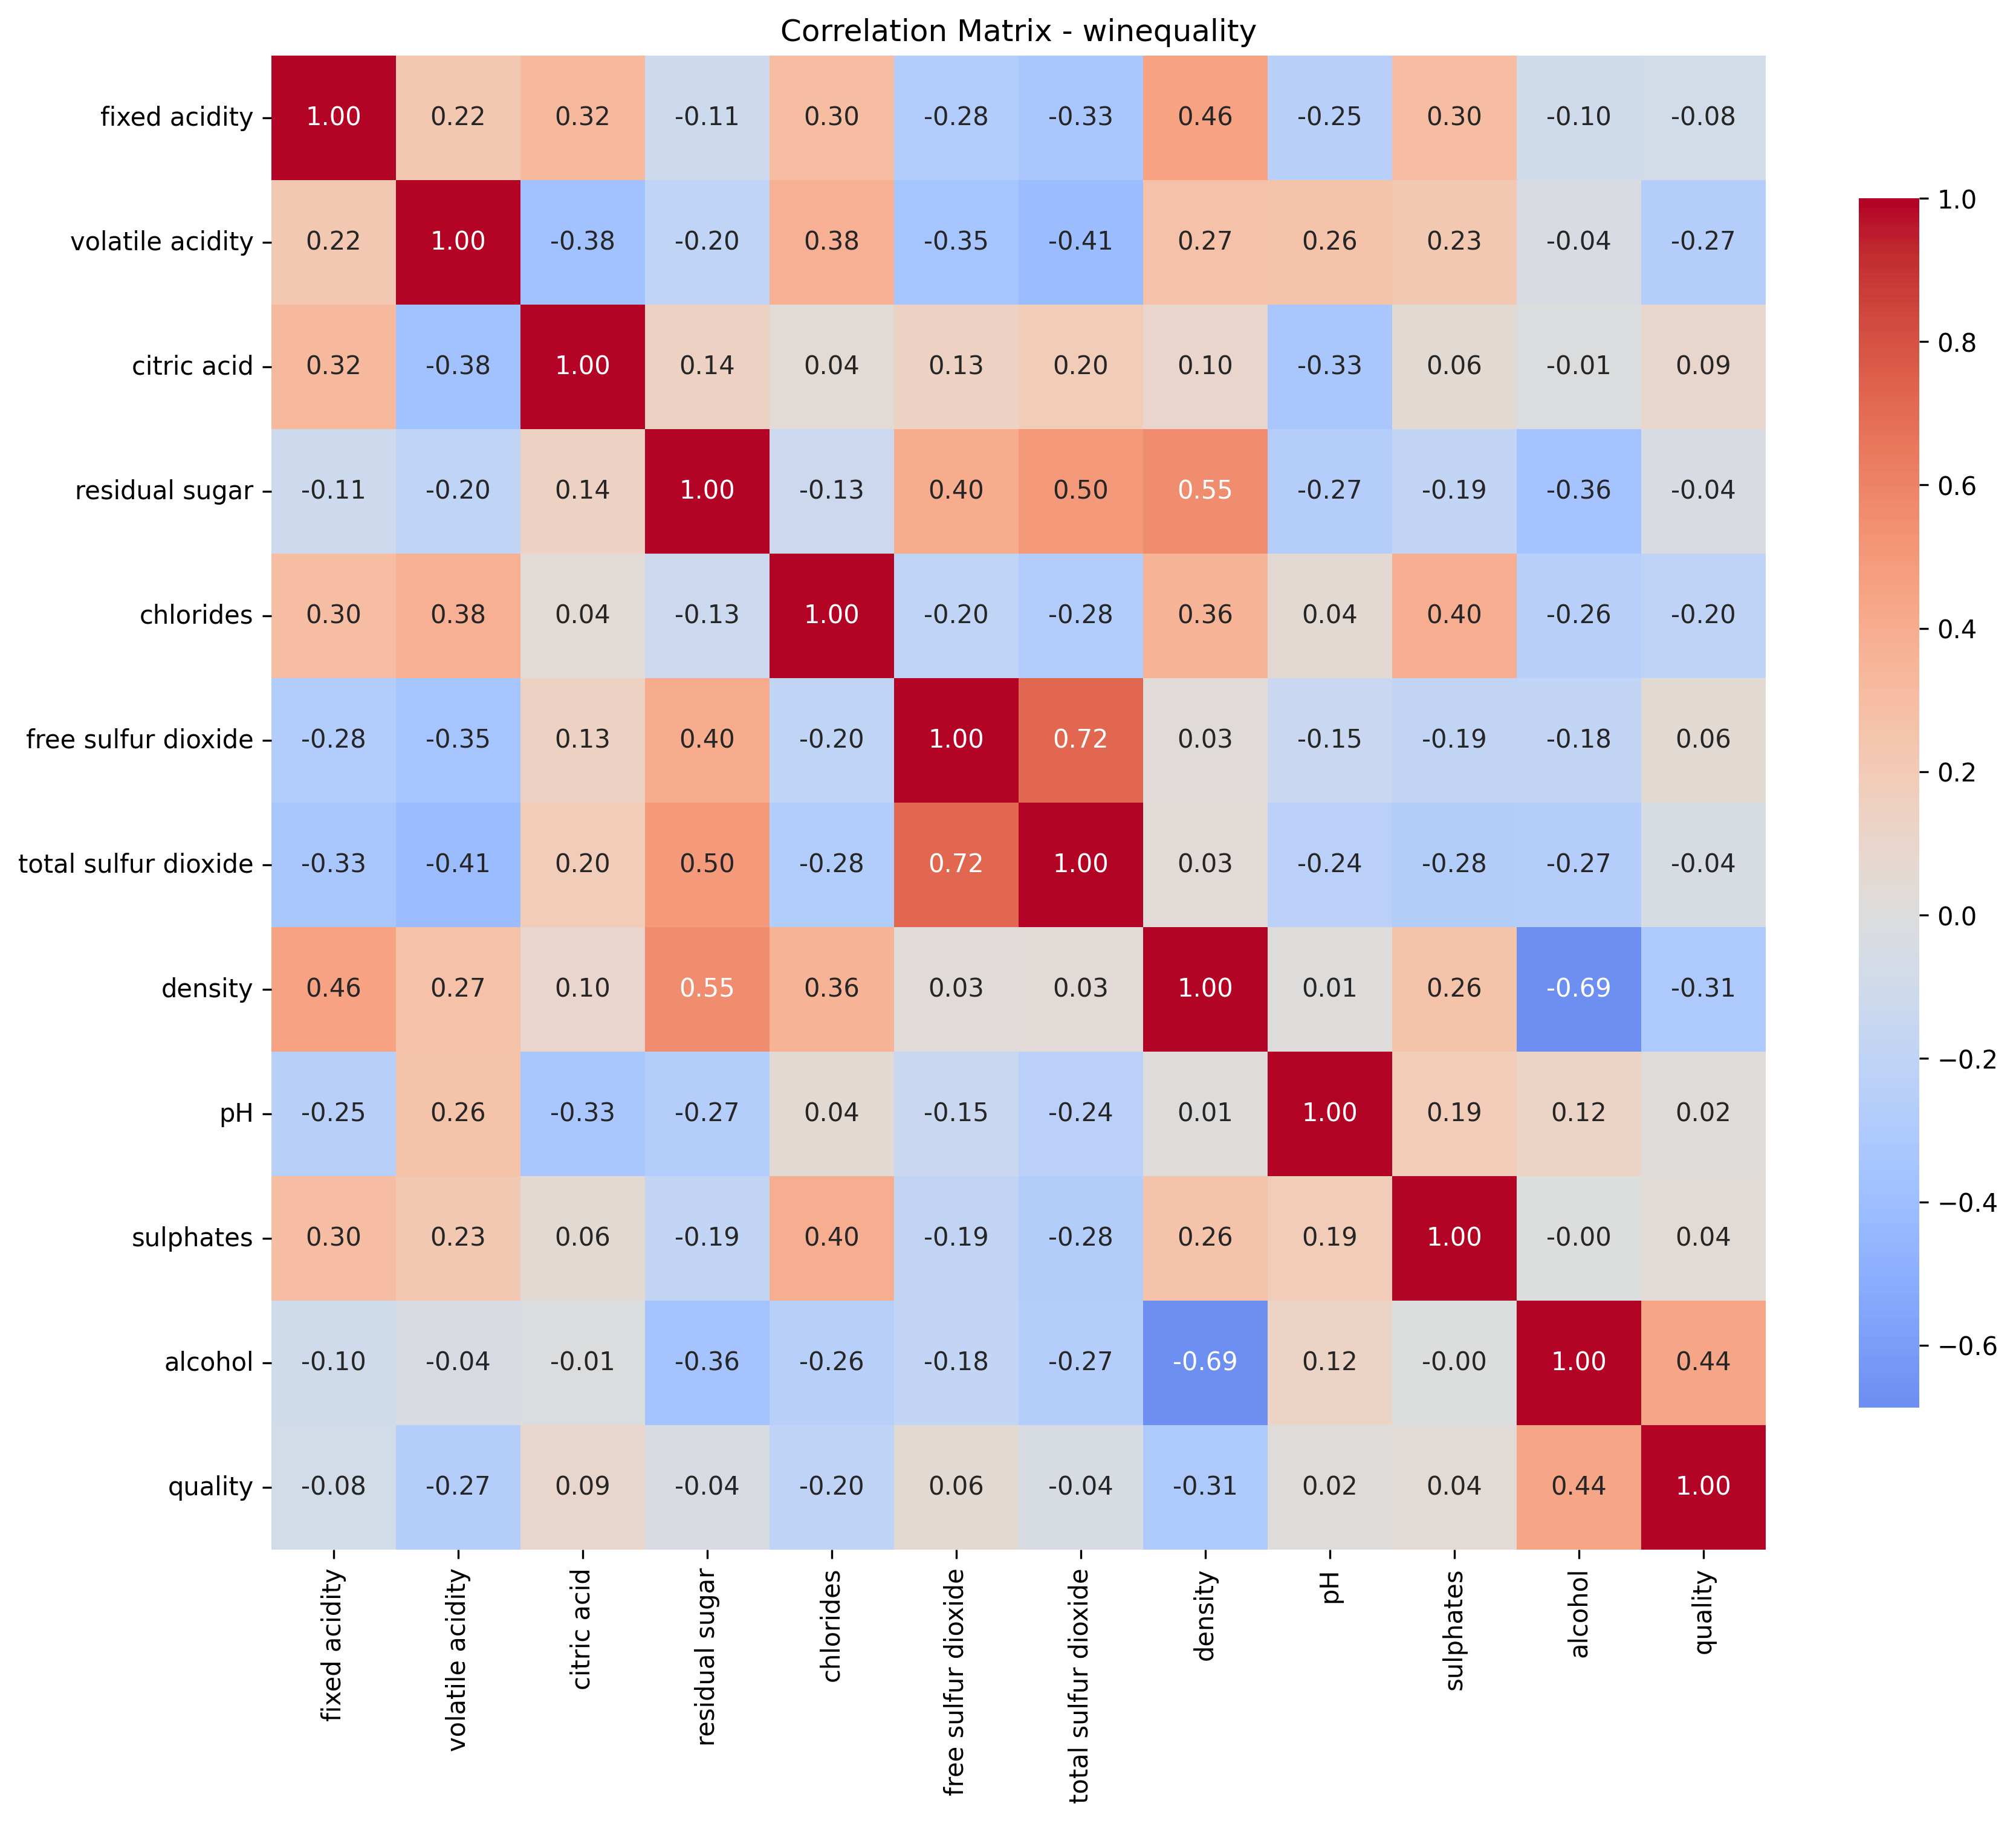
\includegraphics[width=0.7\textwidth]{images/correlation_heatmap_winequality.png}
\caption{Корреляционная матрица — Wine Quality Dataset}
\end{figure}

\subsection{Распределения целевых переменных}

Распределения целевых переменных показывают характер задач для каждого датасета.

\begin{figure}[H]
\centering
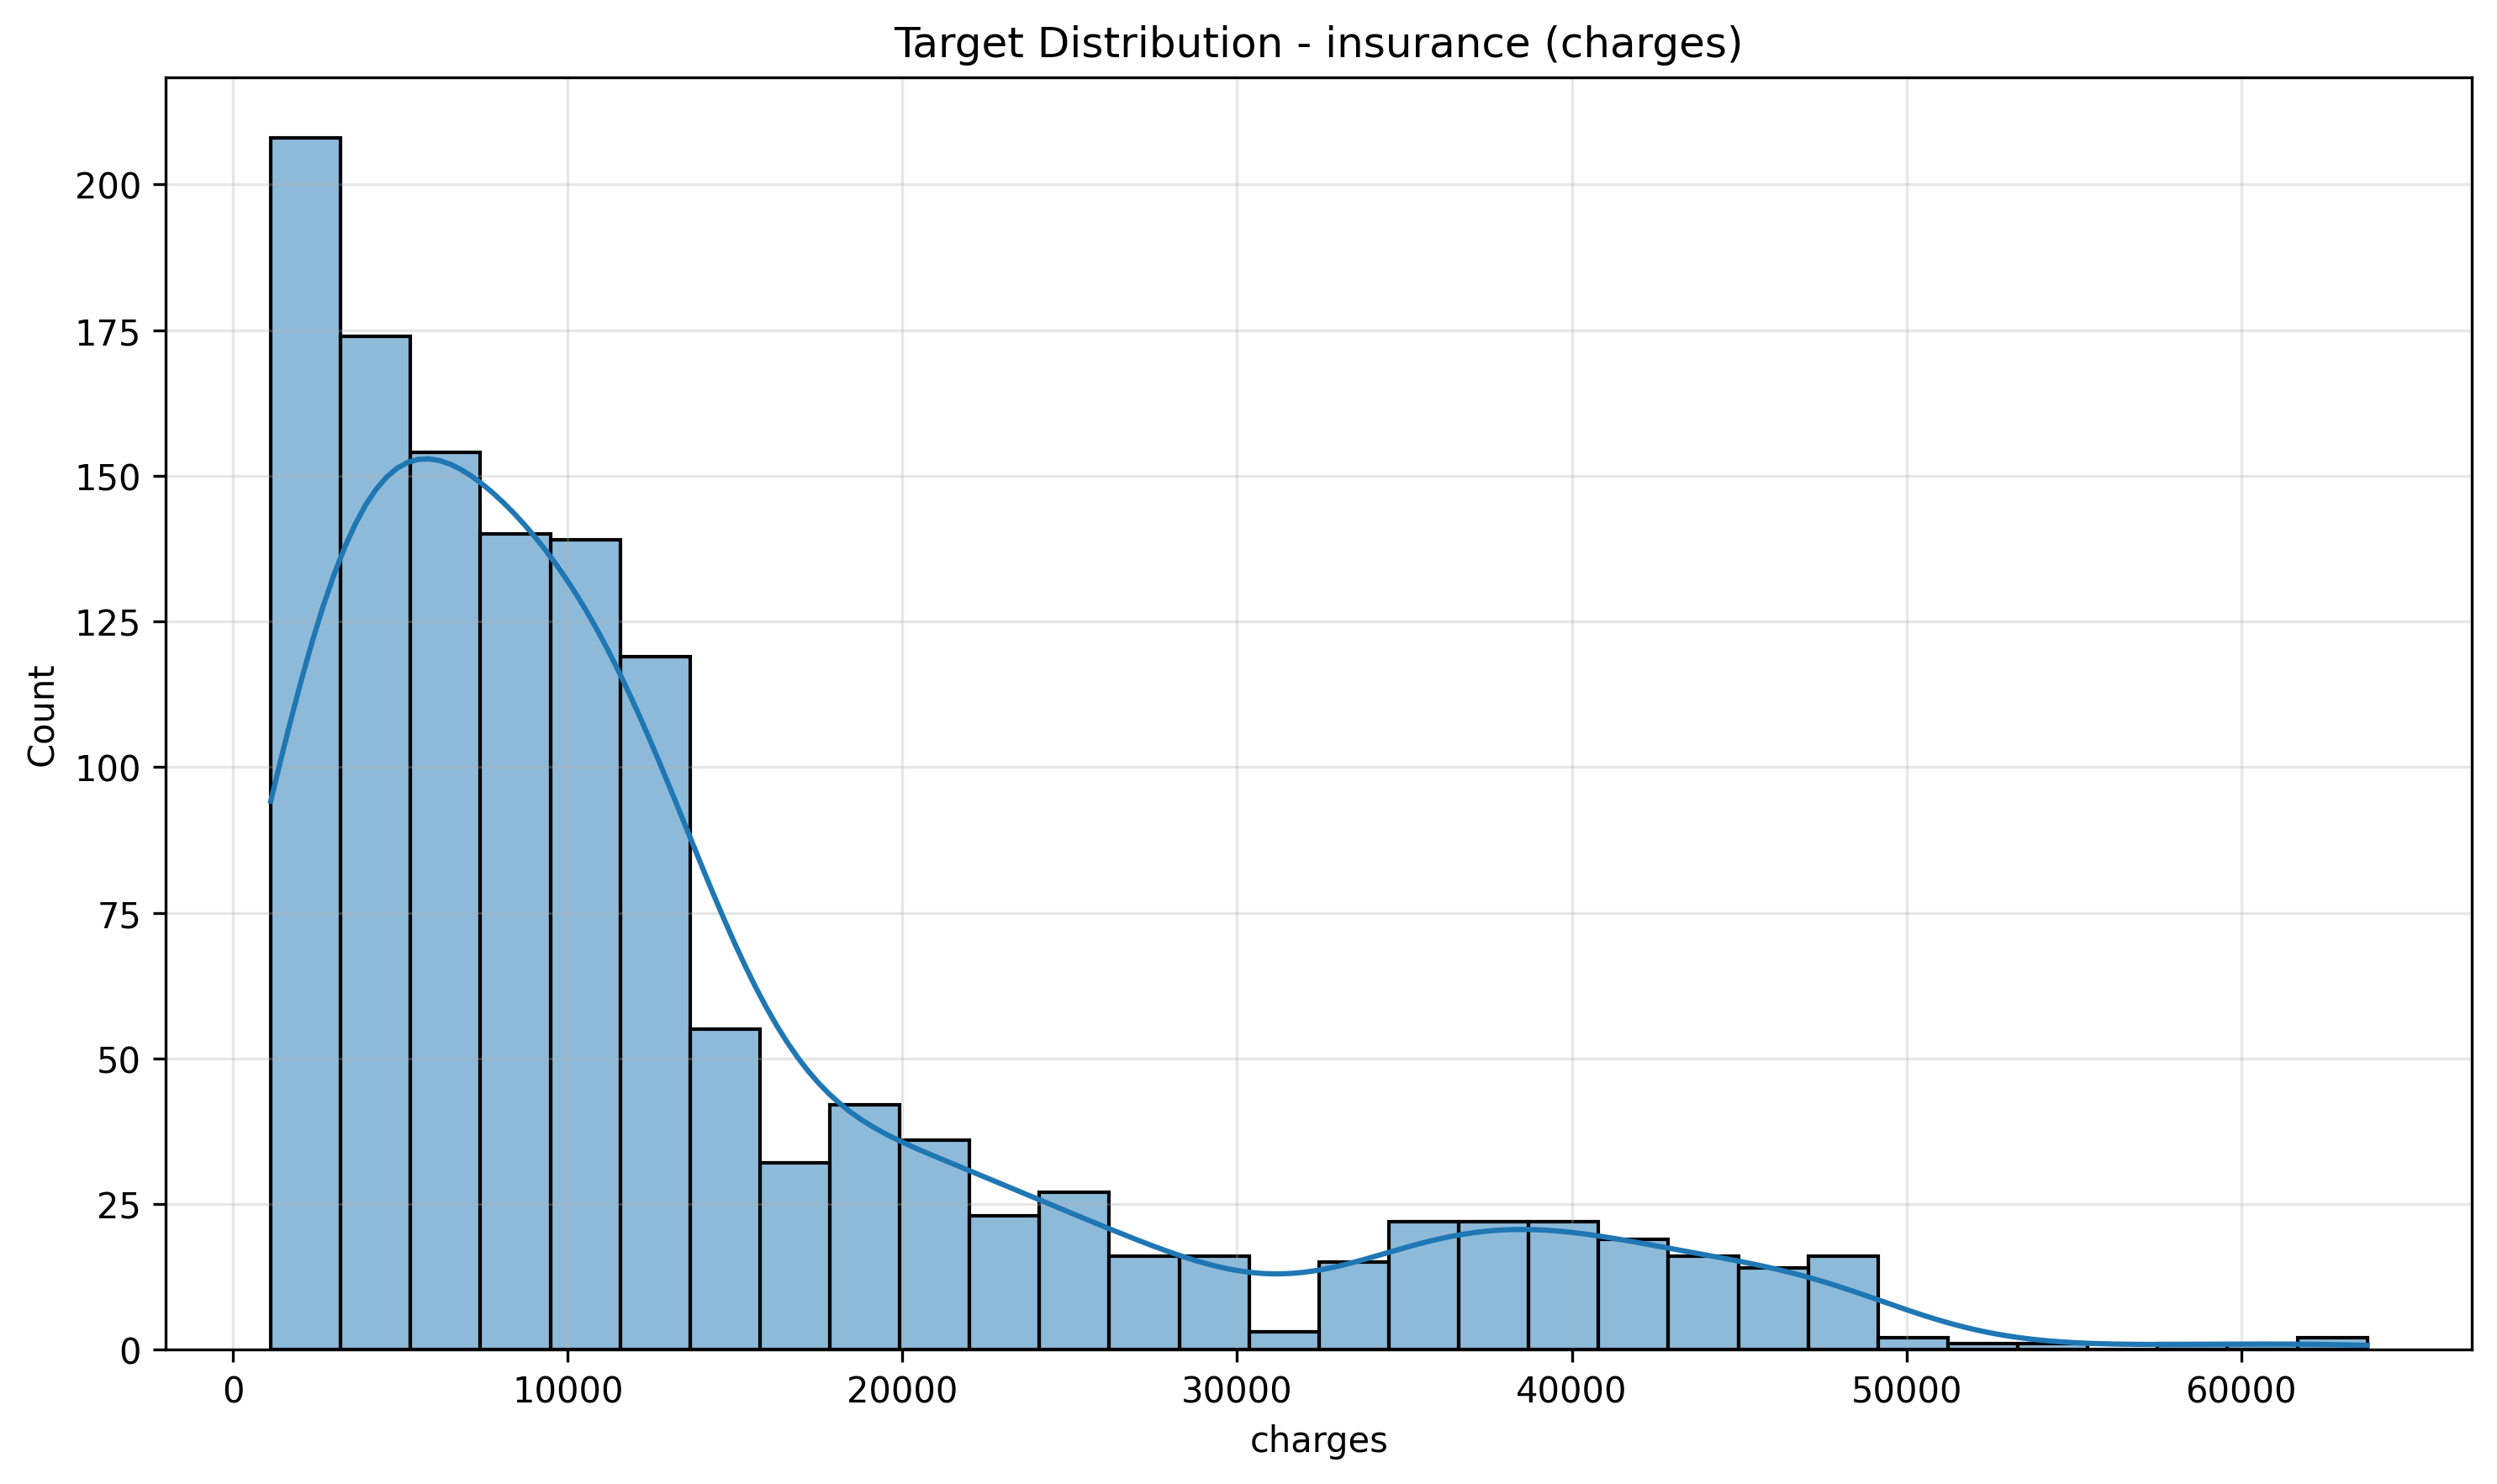
\includegraphics[width=0.7\textwidth]{images/target_distribution_insurance.png}
\caption{Распределение стоимости страховки (Insurance)}
\end{figure}

\begin{figure}[H]
\centering
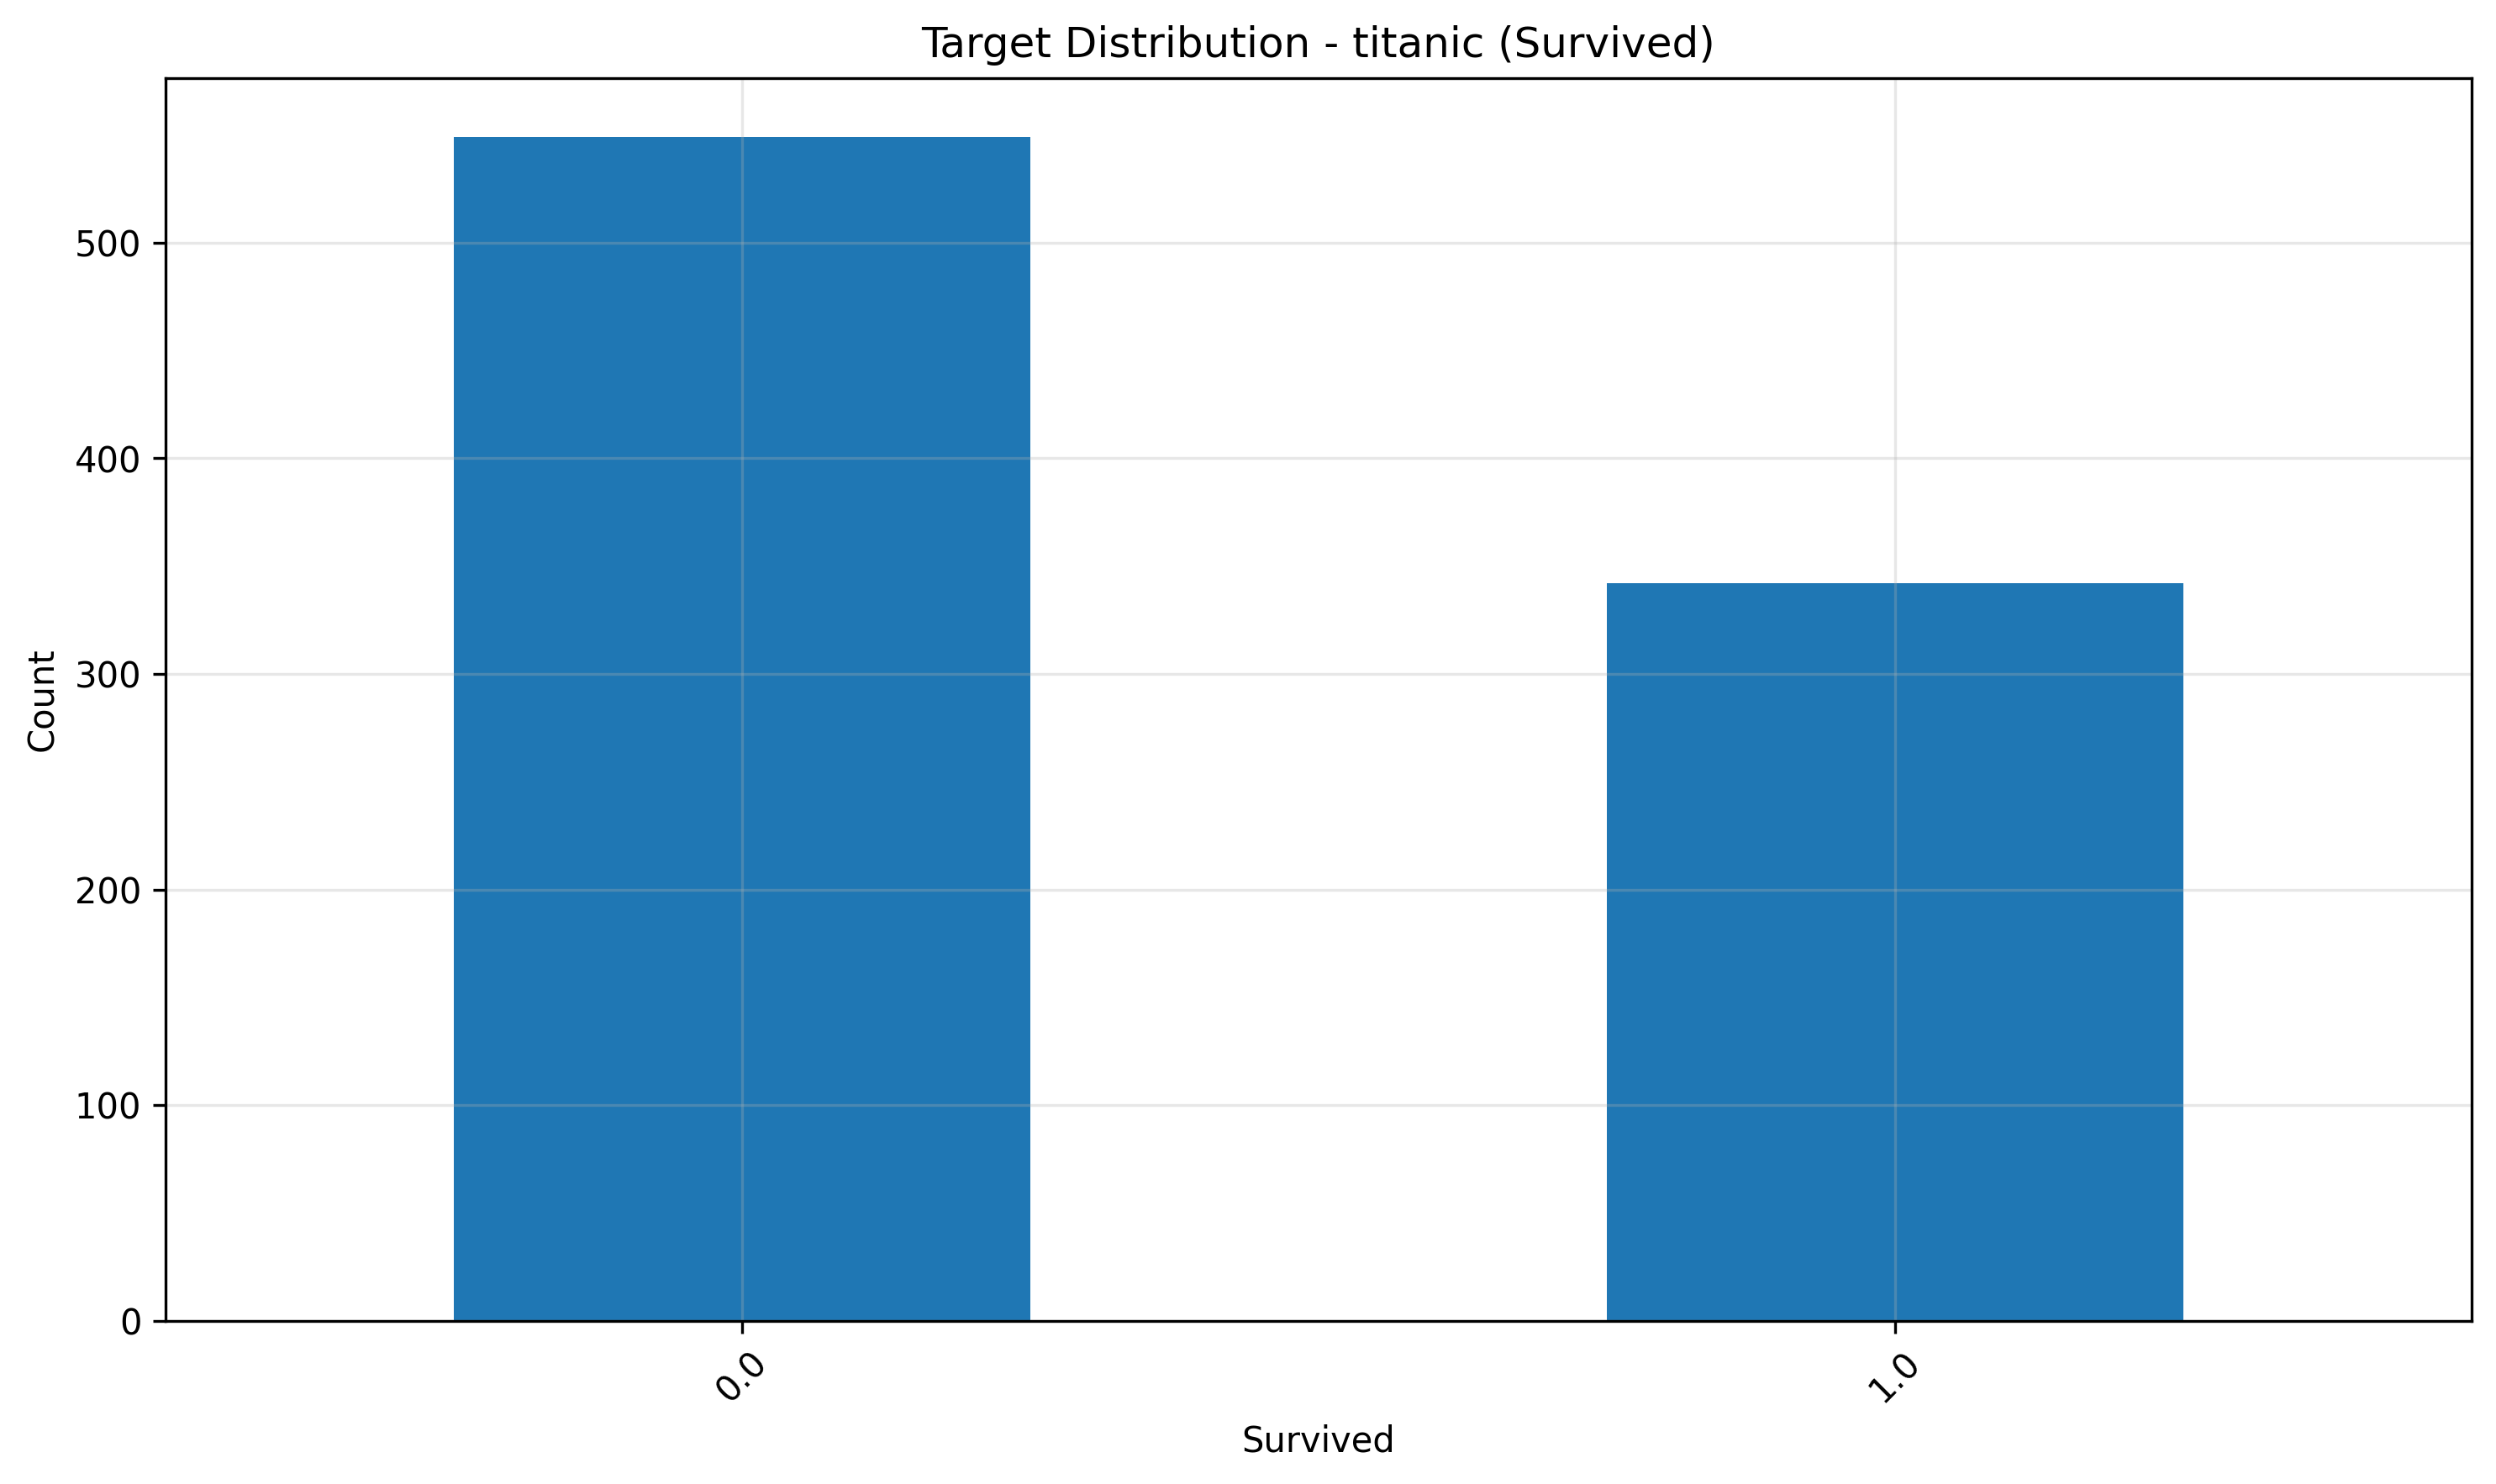
\includegraphics[width=0.7\textwidth]{images/target_distribution_titanic.png}
\caption{Распределение выживаемости (Titanic)}
\end{figure}

\begin{figure}[H]
\centering
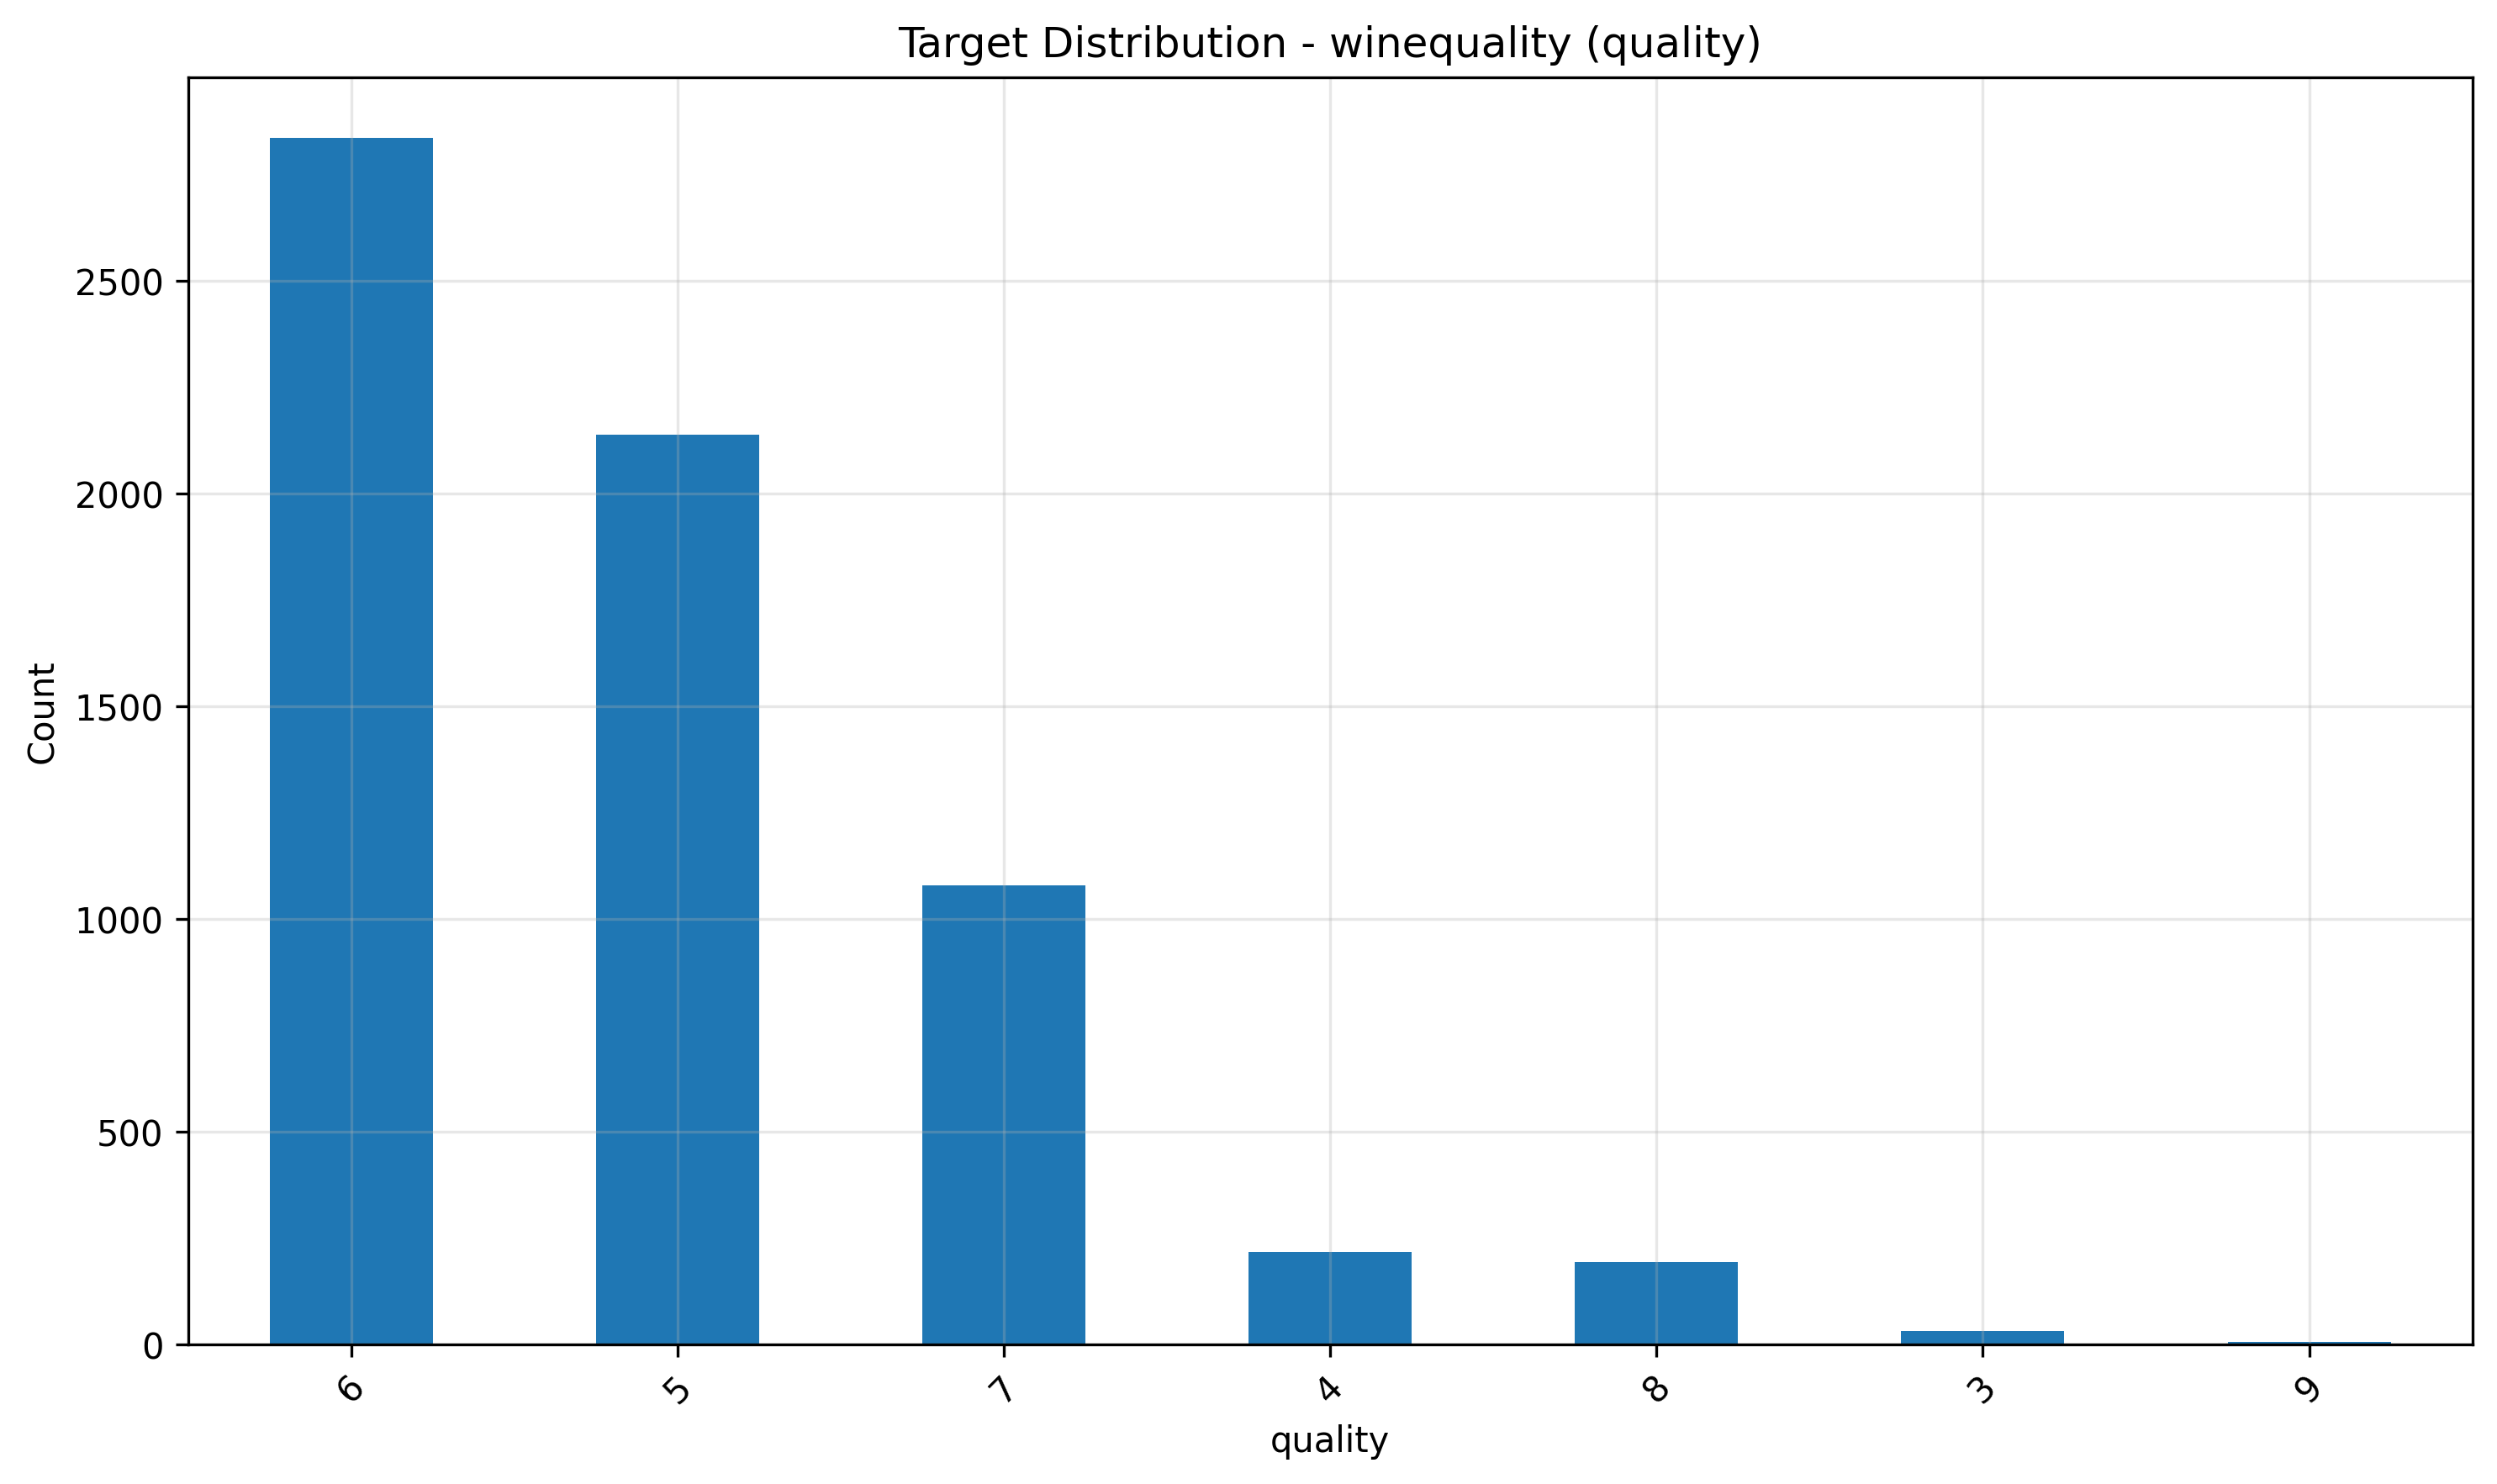
\includegraphics[width=0.7\textwidth]{images/target_distribution_winequality.png}
\caption{Распределение качества вина (Wine Quality)}
\end{figure}

\subsection{Примеры гистограмм признаков}

\begin{figure}[H]
\centering
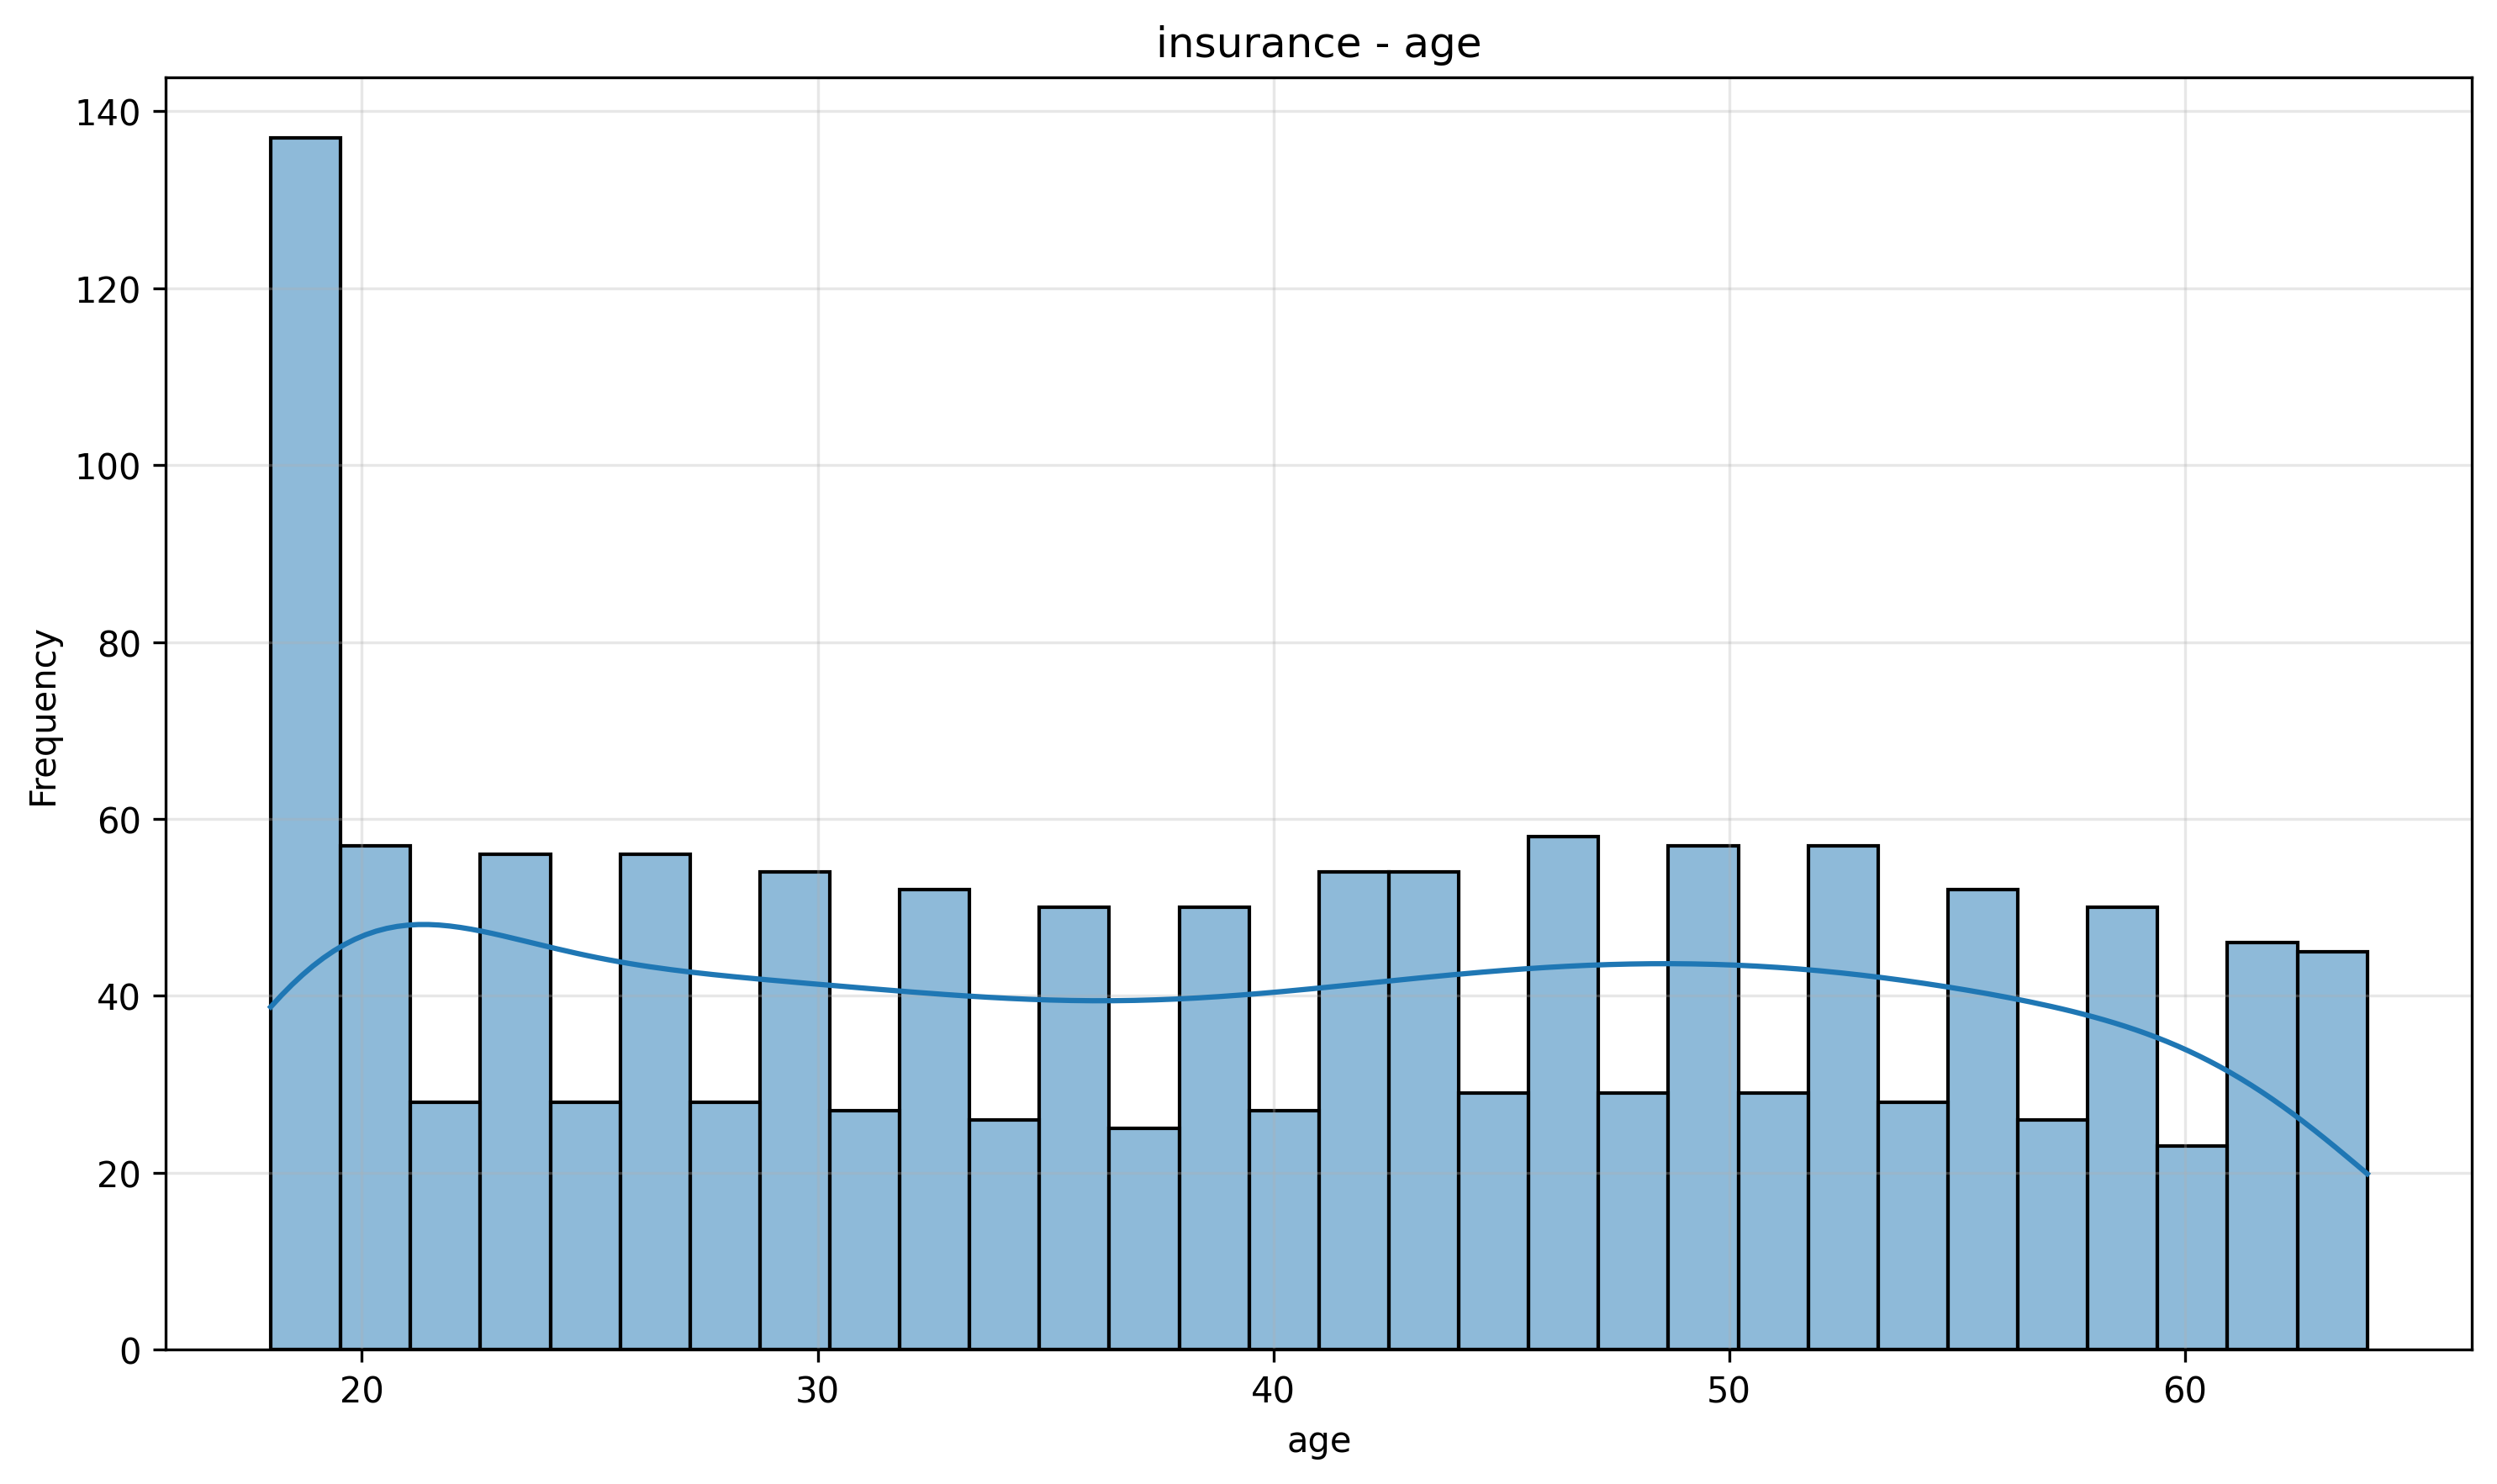
\includegraphics[width=0.7\textwidth]{images/hist_insurance_age.png}
\caption{Распределение возраста — Insurance Dataset}
\end{figure}

\begin{figure}[H]
\centering
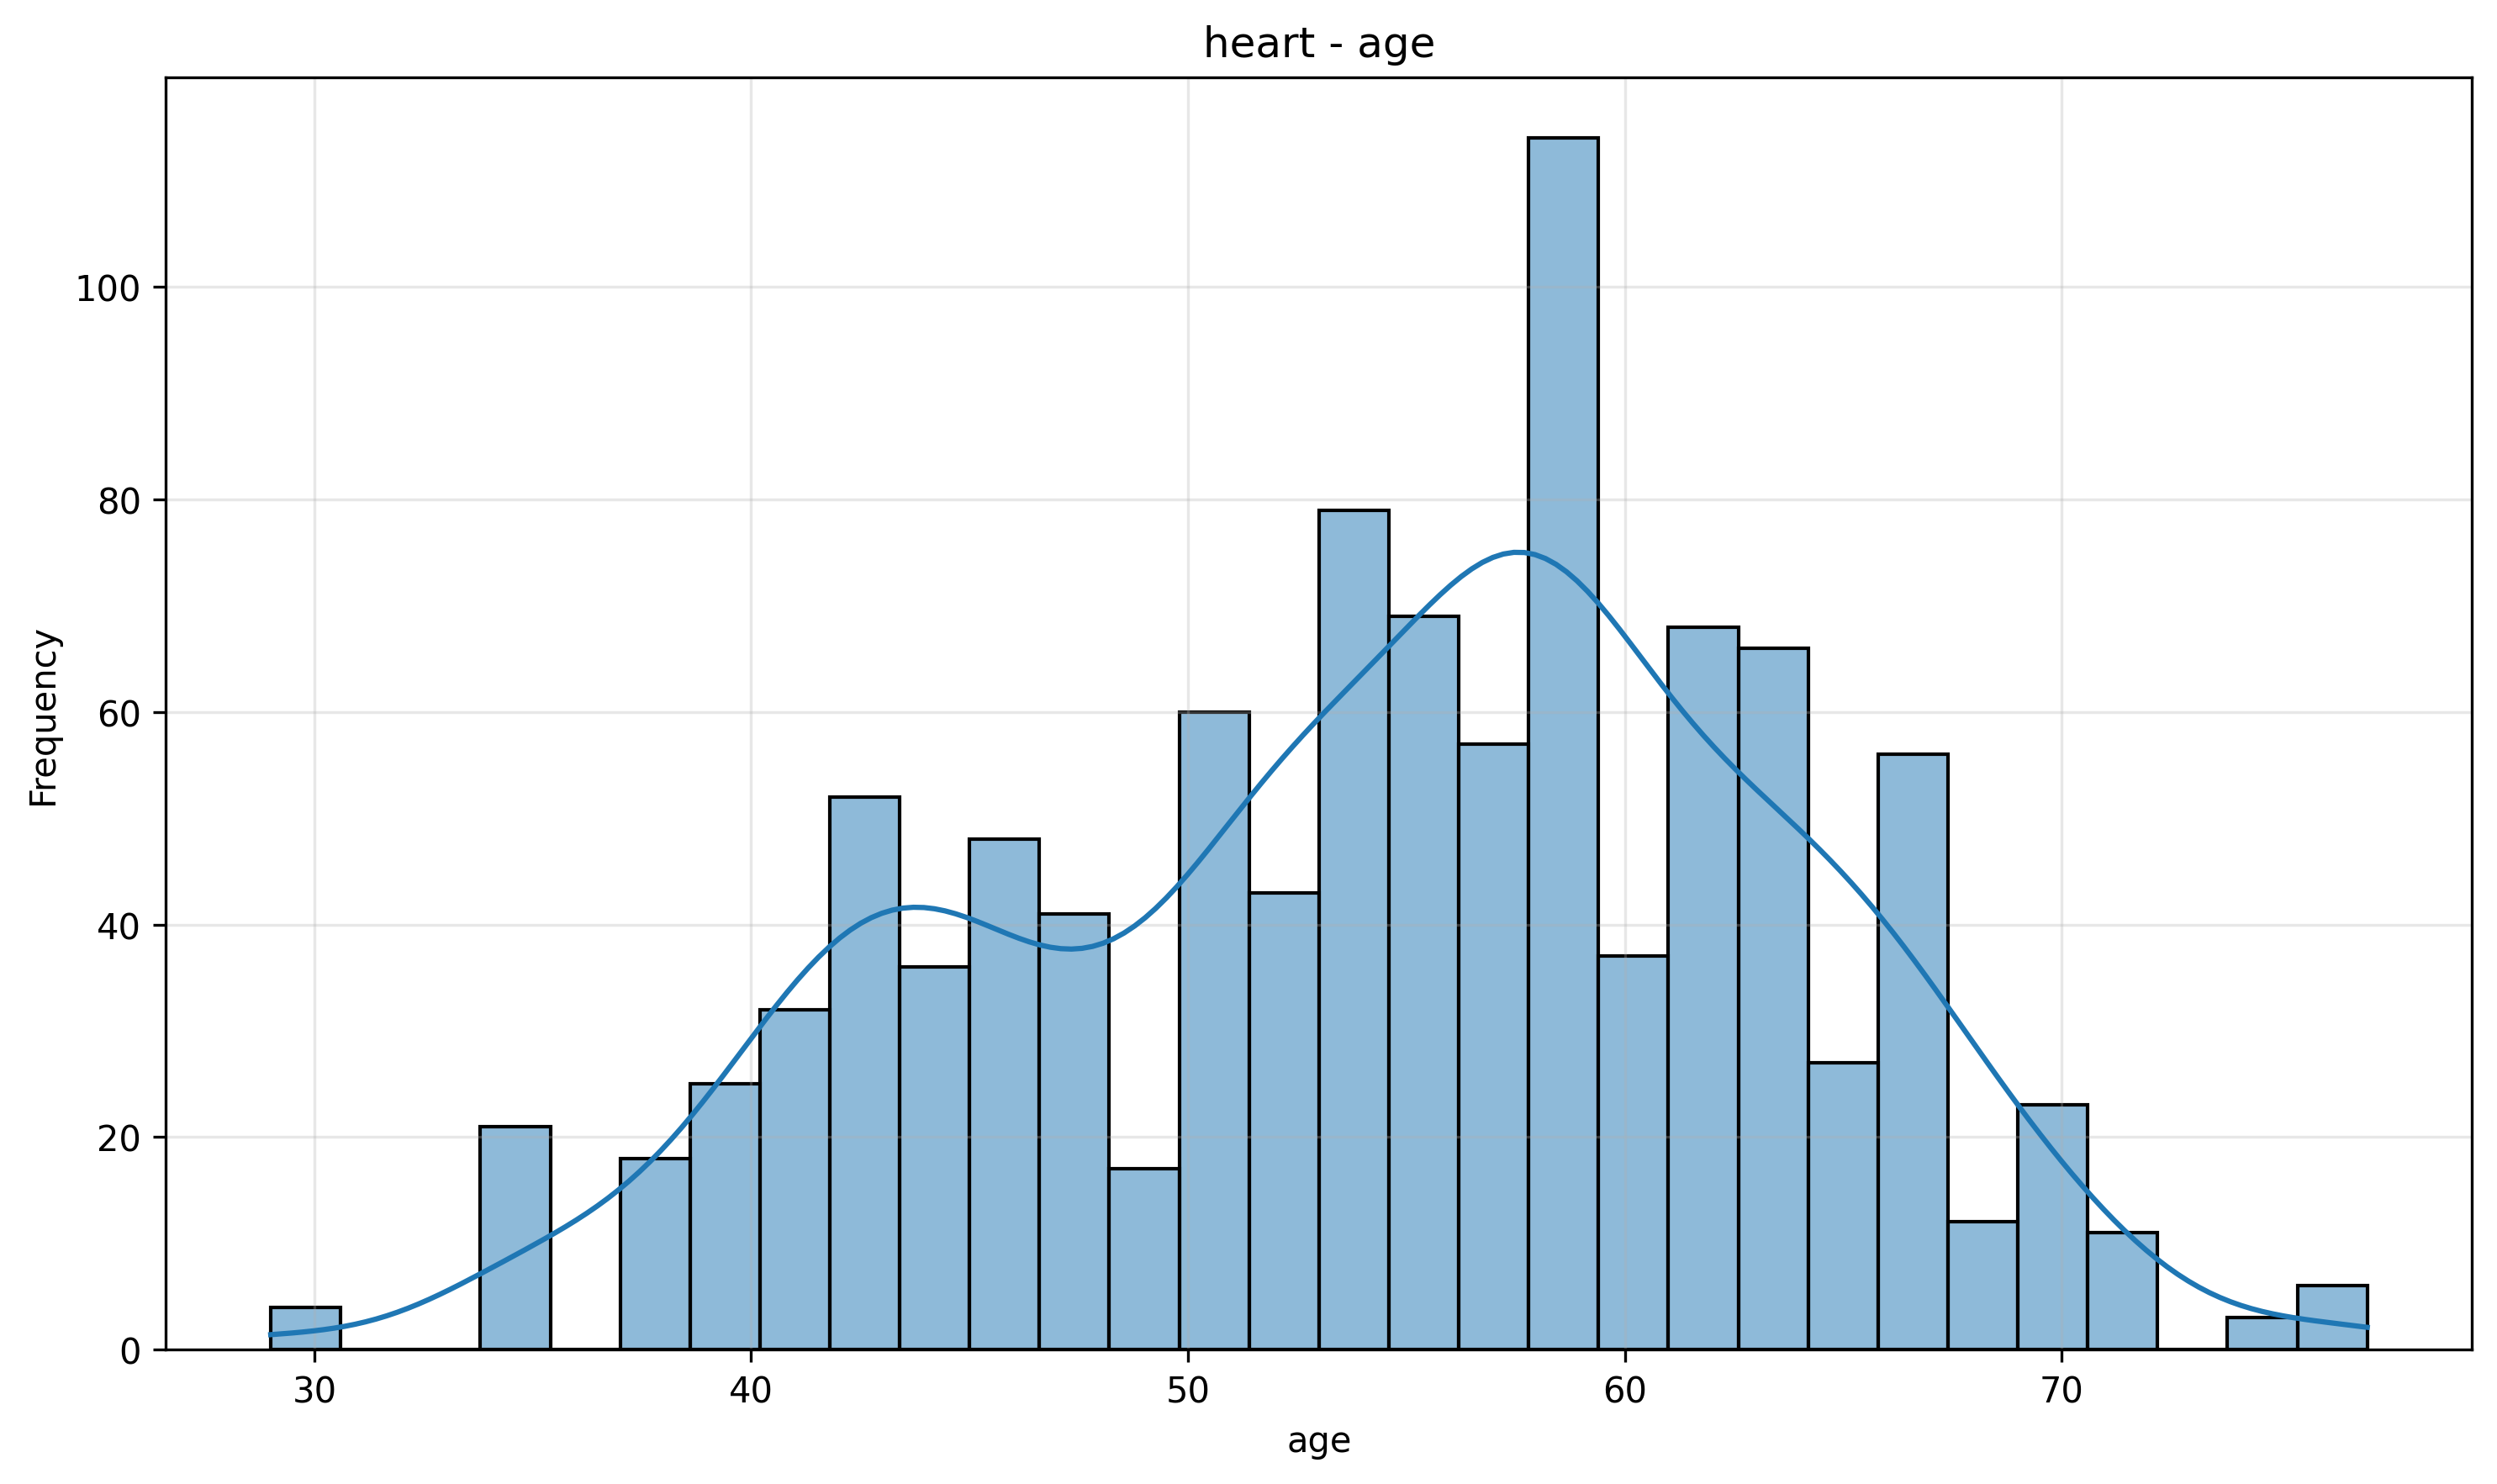
\includegraphics[width=0.7\textwidth]{images/hist_heart_age.png}
\caption{Распределение возраста — Heart Disease Dataset}
\end{figure}

\subsection{ROC-кривые для моделей классификации}

ROC-кривые демонстрируют качество классификации для разных методов.

\begin{figure}[H]
\centering
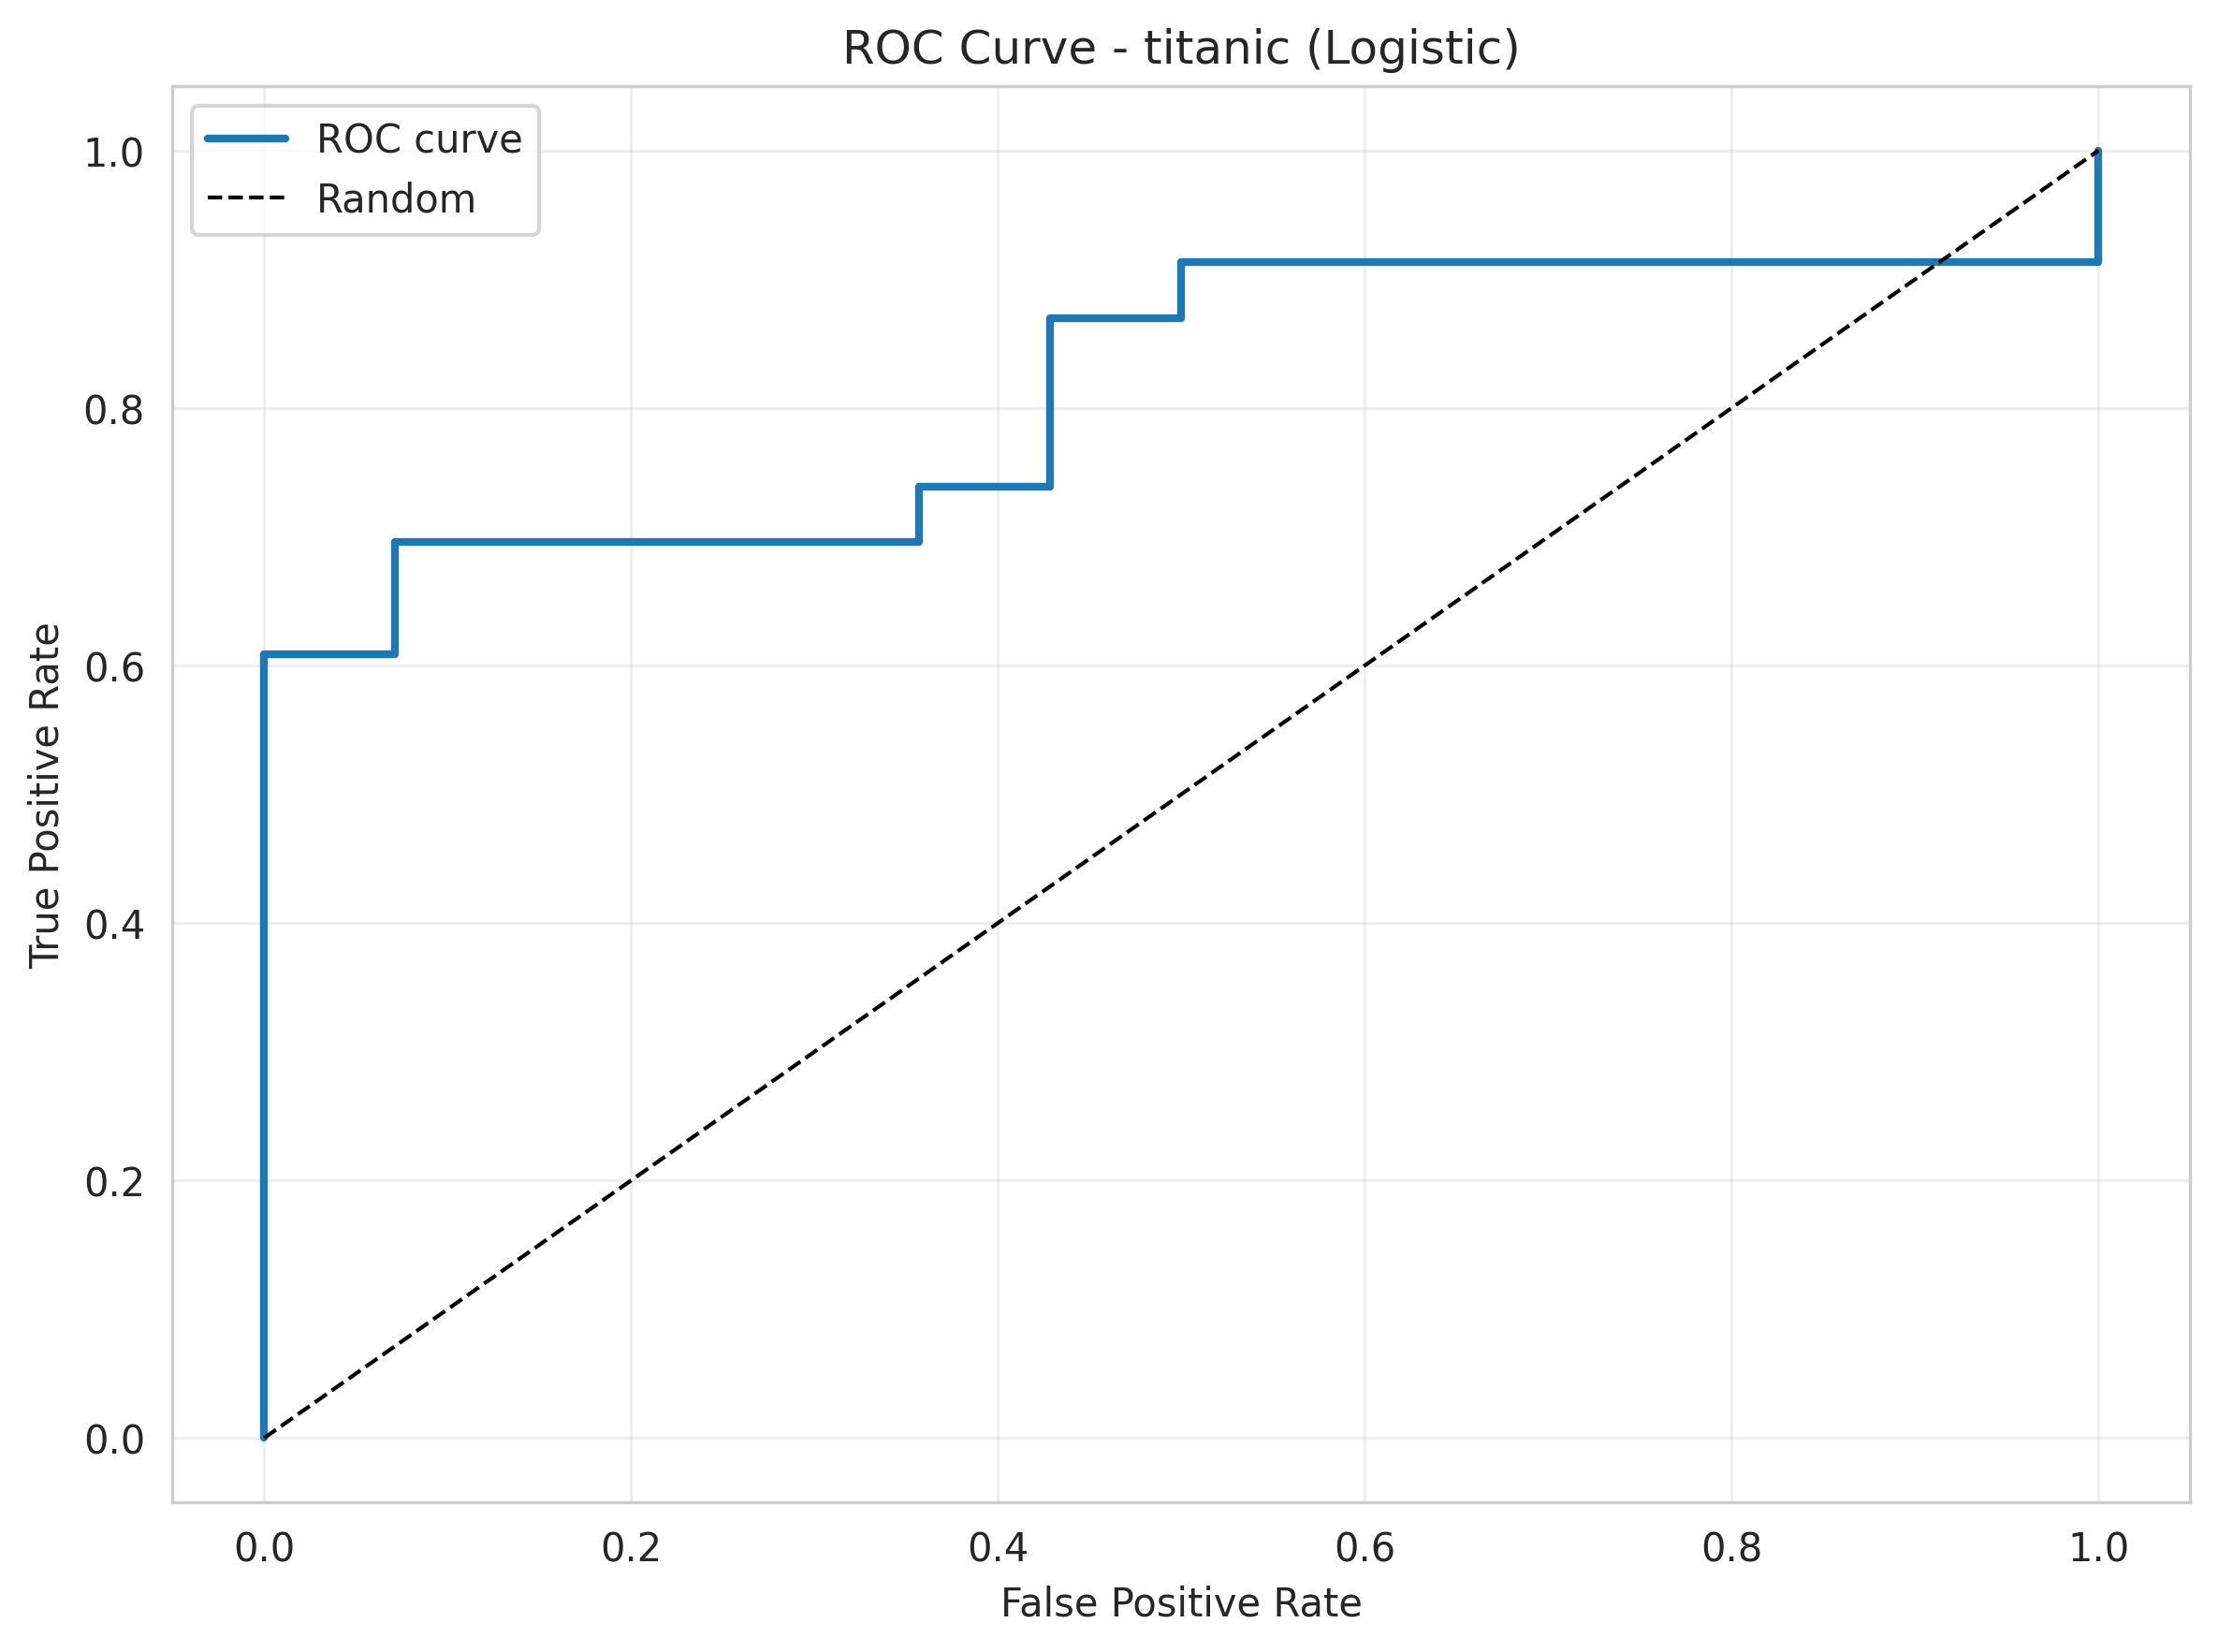
\includegraphics[width=0.7\textwidth]{images/roc_curve_titanic_logistic.png}
\caption{ROC-кривая — Titanic Dataset (Logistic Regression)}
\end{figure}

\begin{figure}[H]
\centering
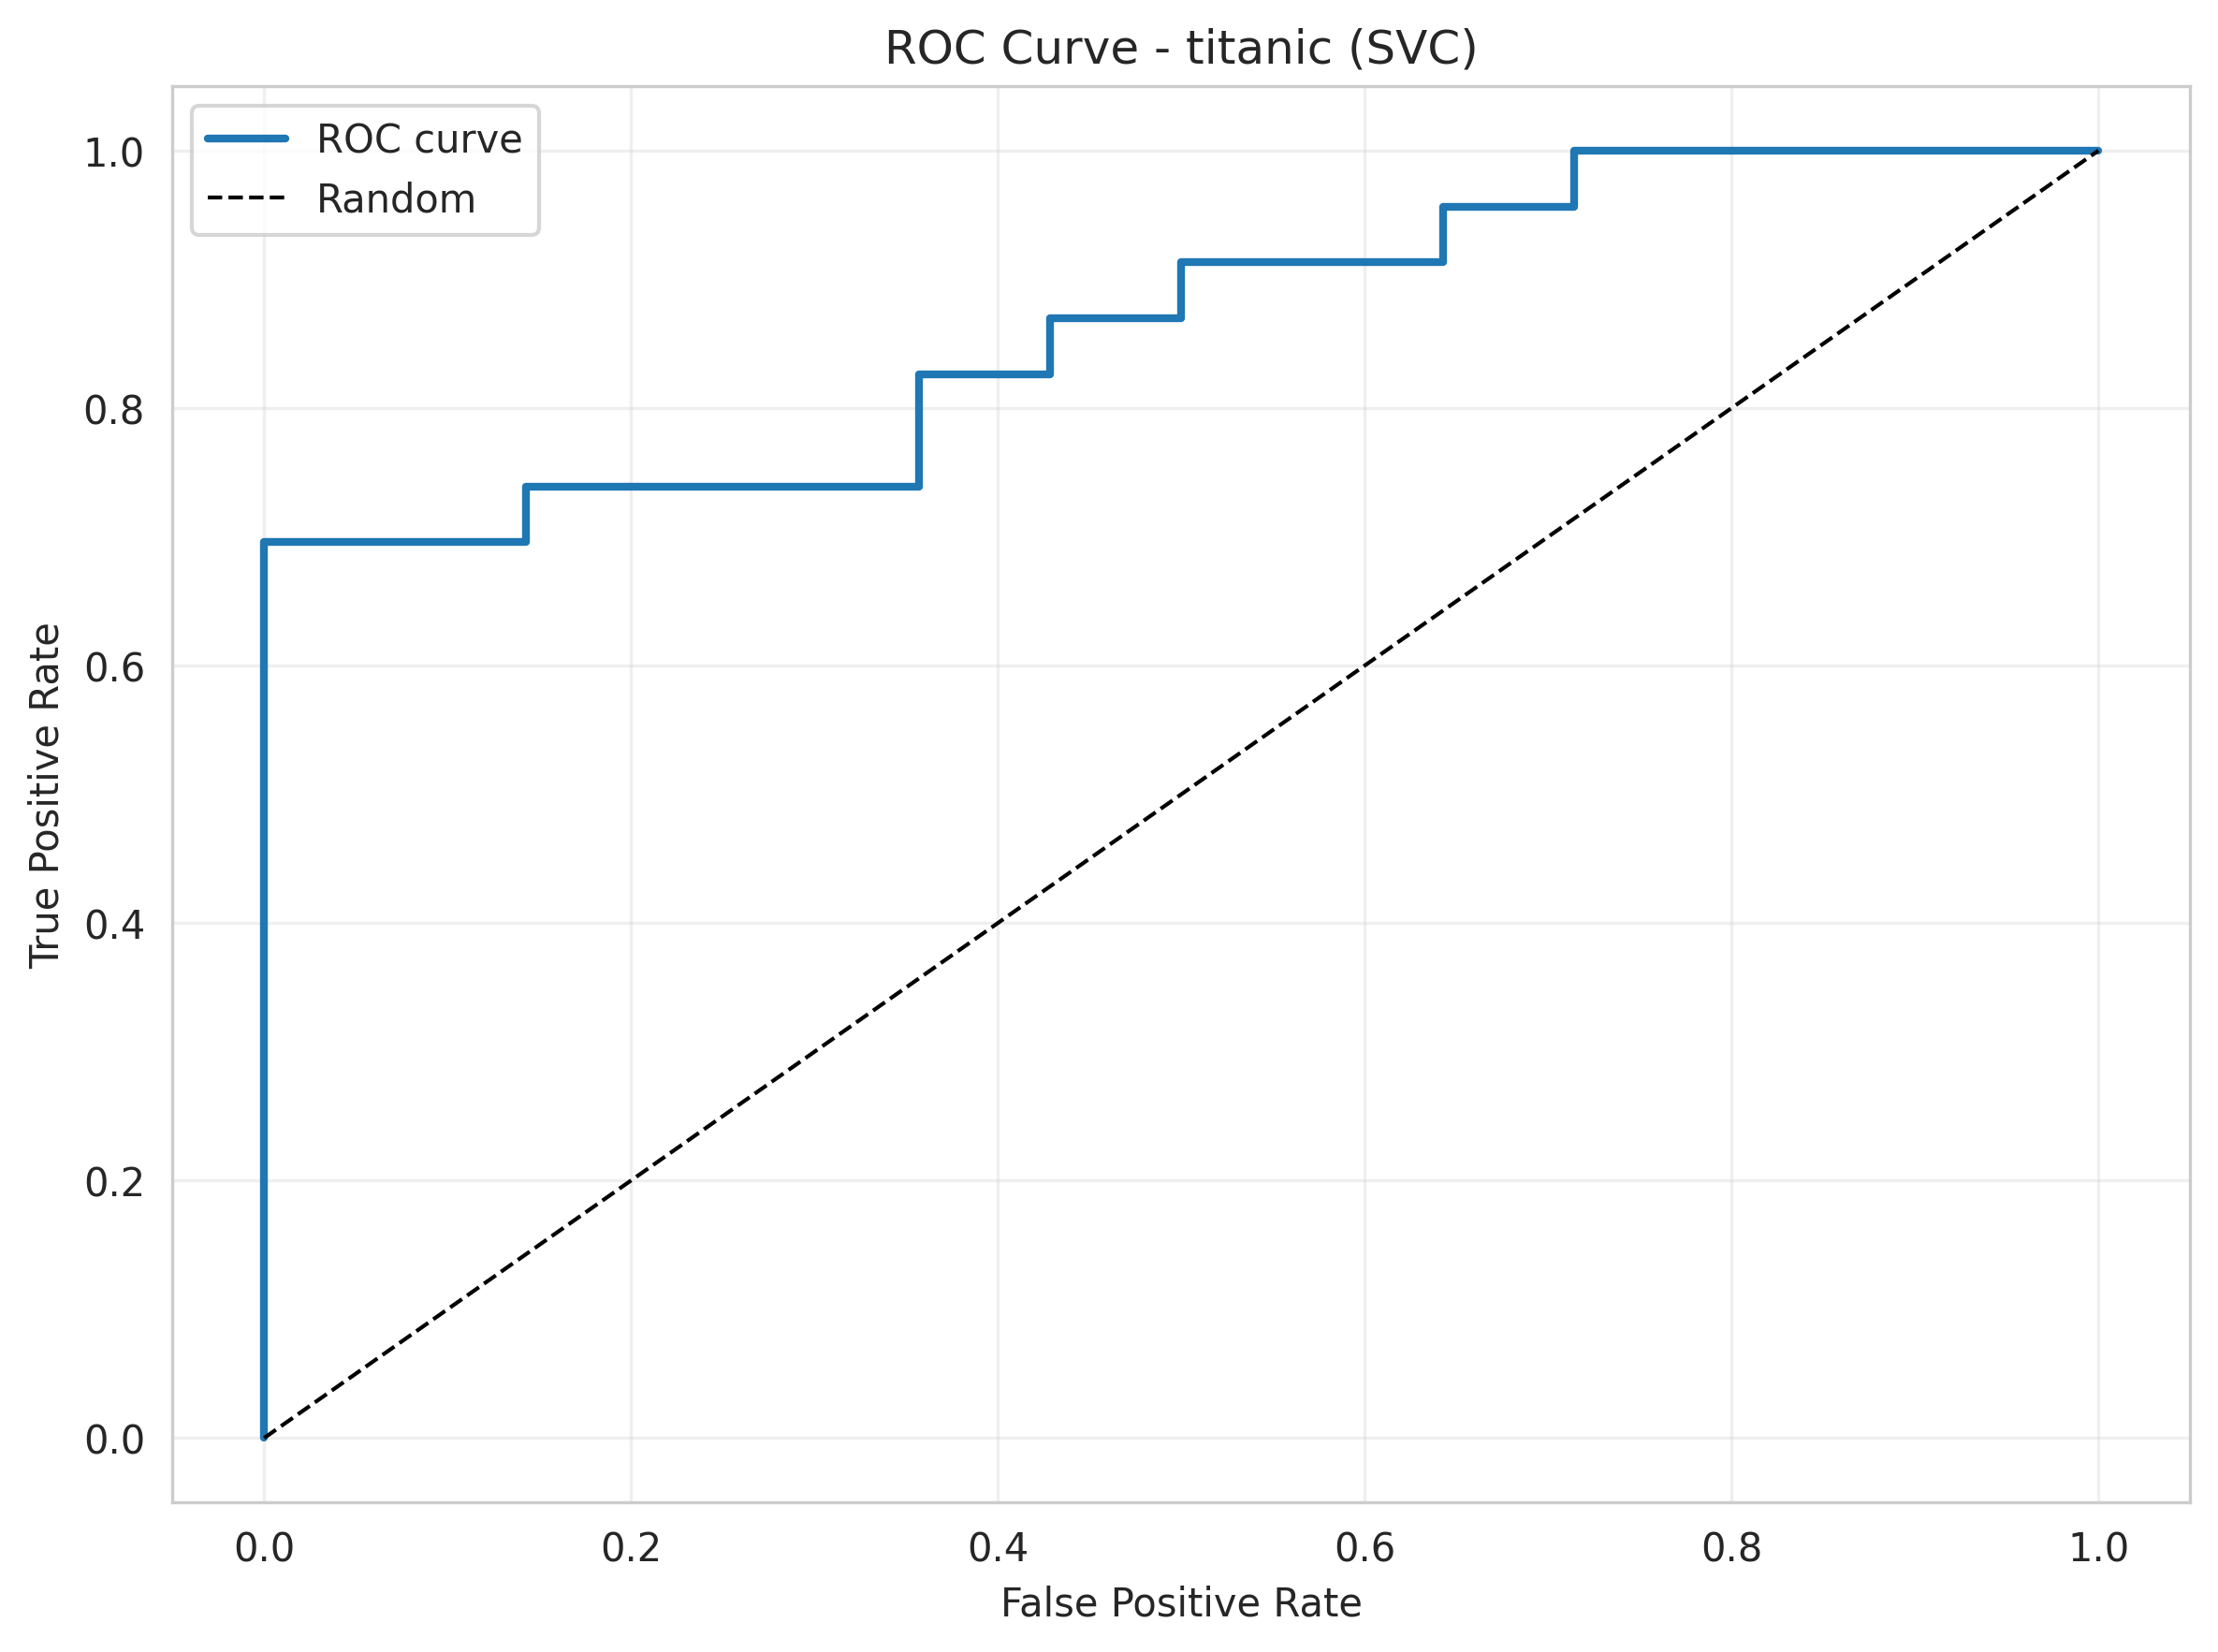
\includegraphics[width=0.7\textwidth]{images/roc_curve_titanic_svc.png}
\caption{ROC-кривая — Titanic Dataset (SVC)}
\end{figure}

\begin{figure}[H]
\centering
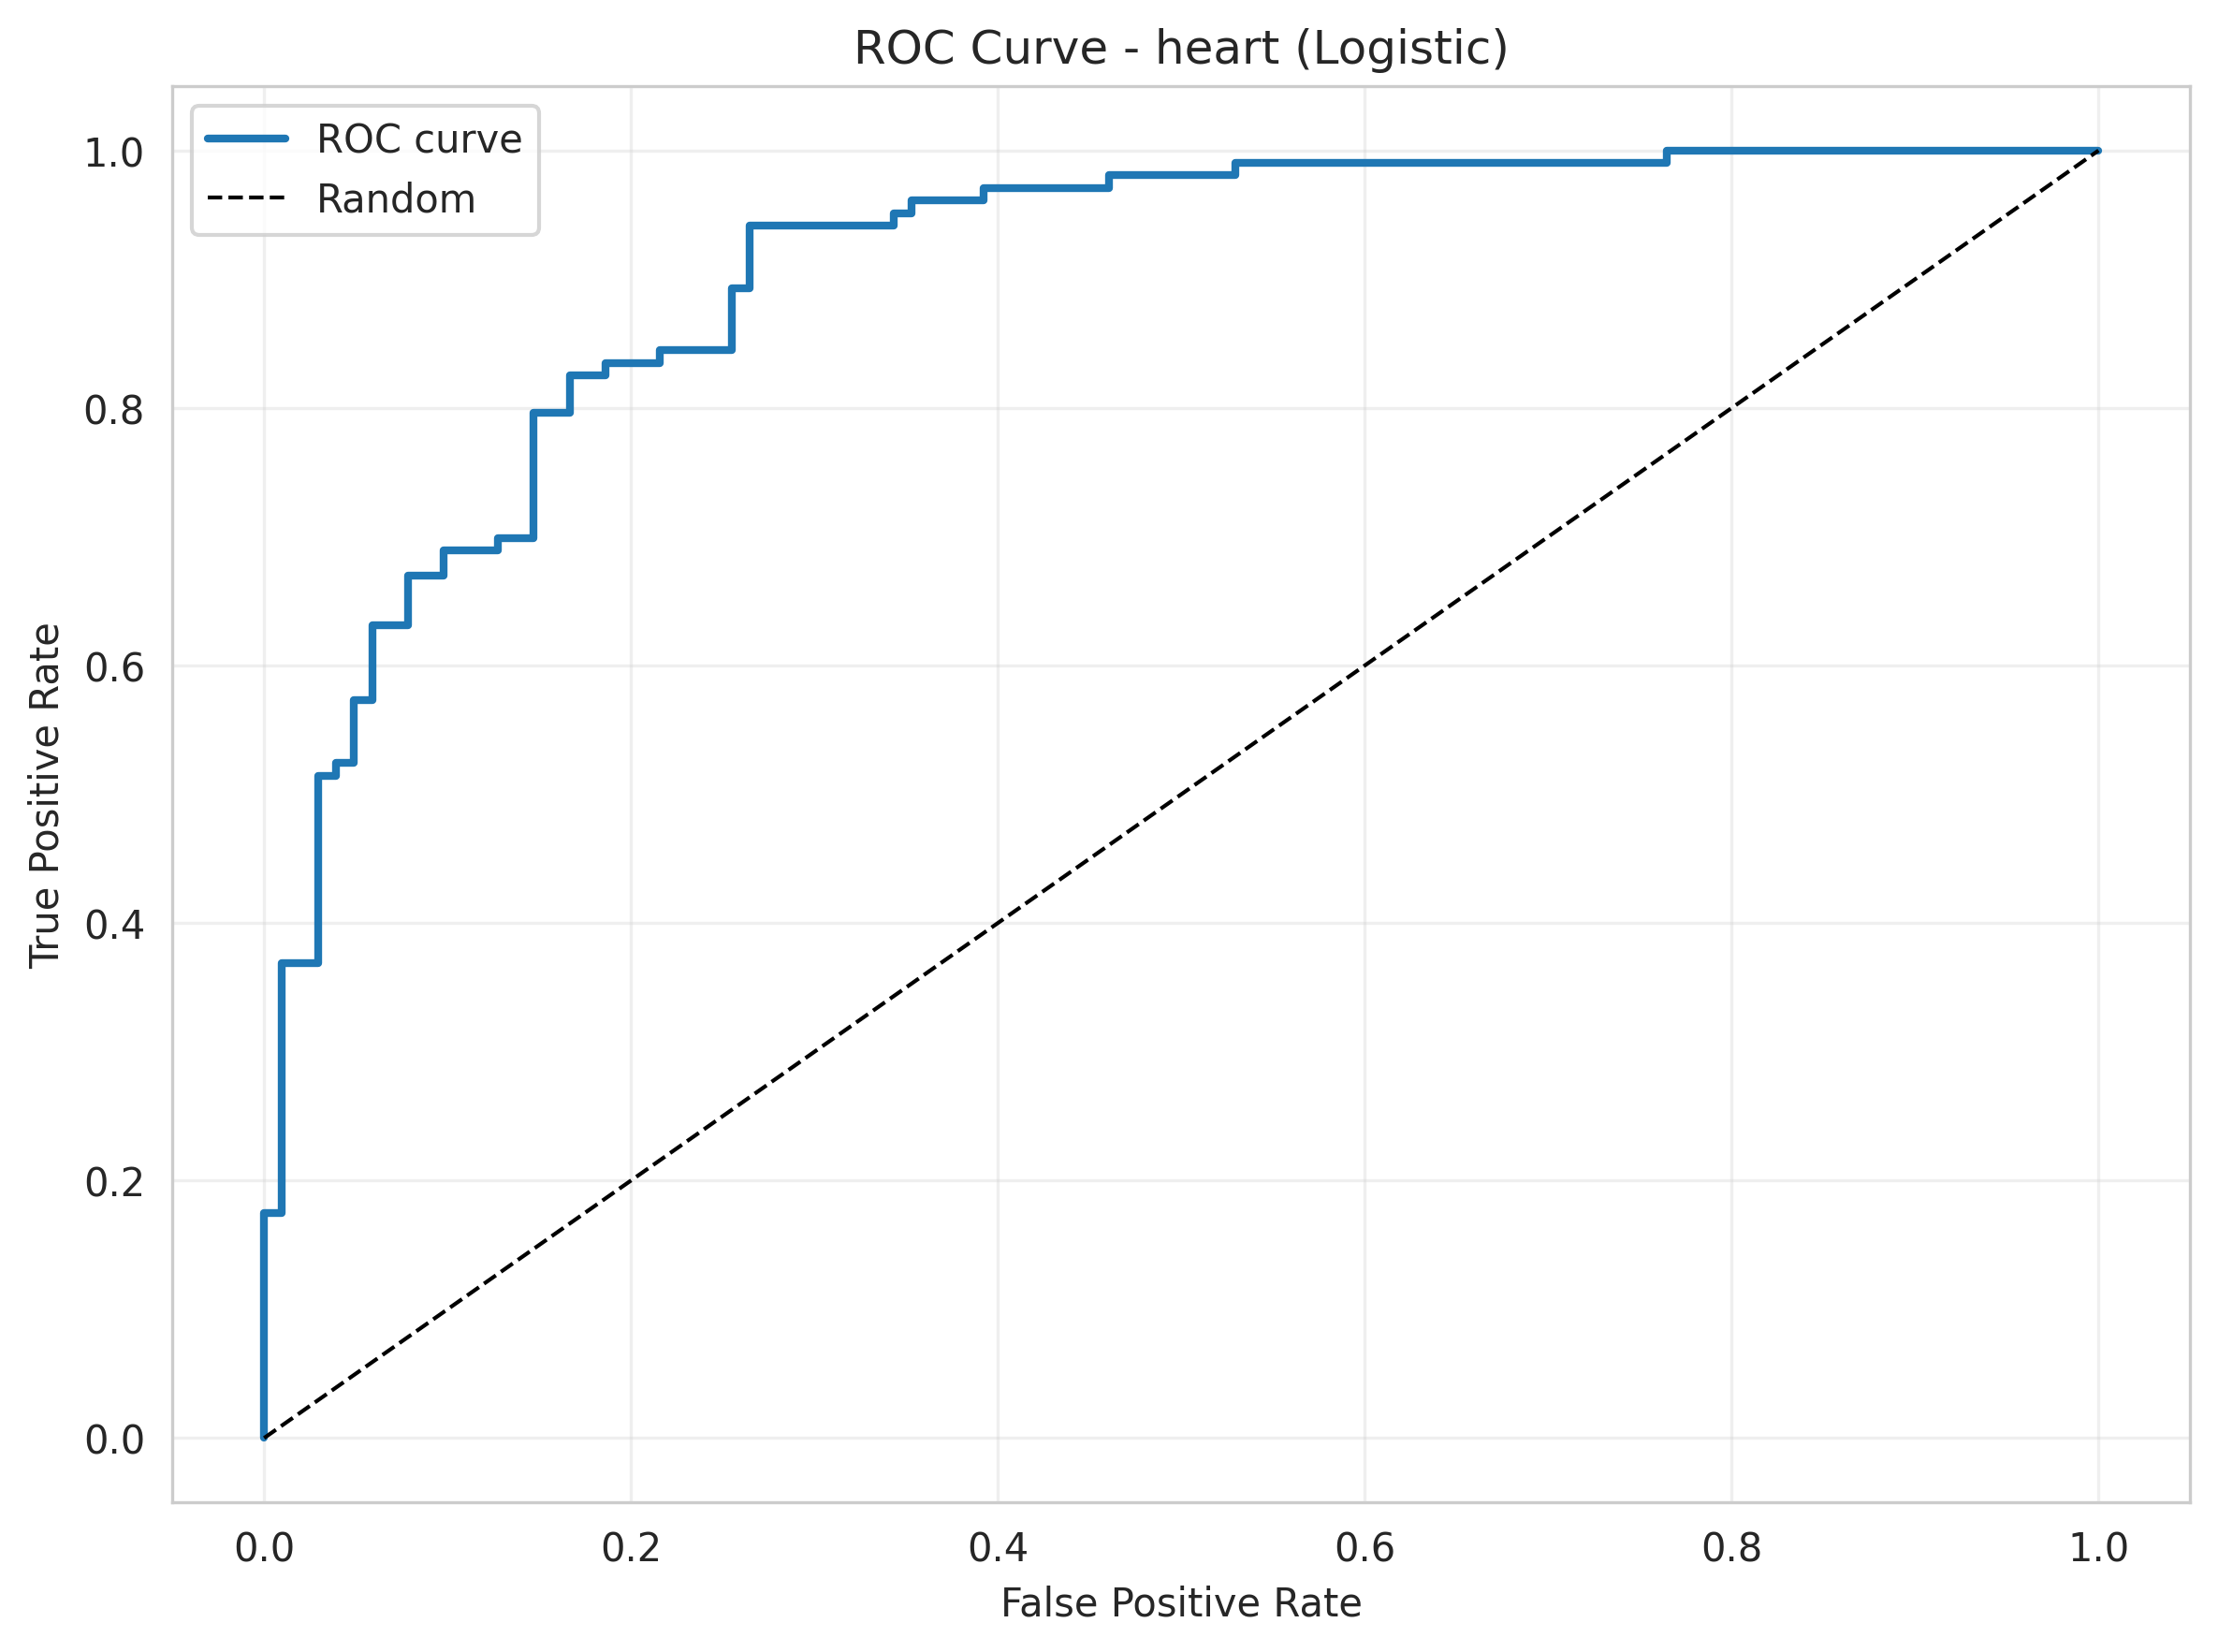
\includegraphics[width=0.7\textwidth]{images/roc_curve_heart_logistic.png}
\caption{ROC-кривая — Heart Disease Dataset (Logistic Regression)}
\end{figure}

\begin{figure}[H]
\centering
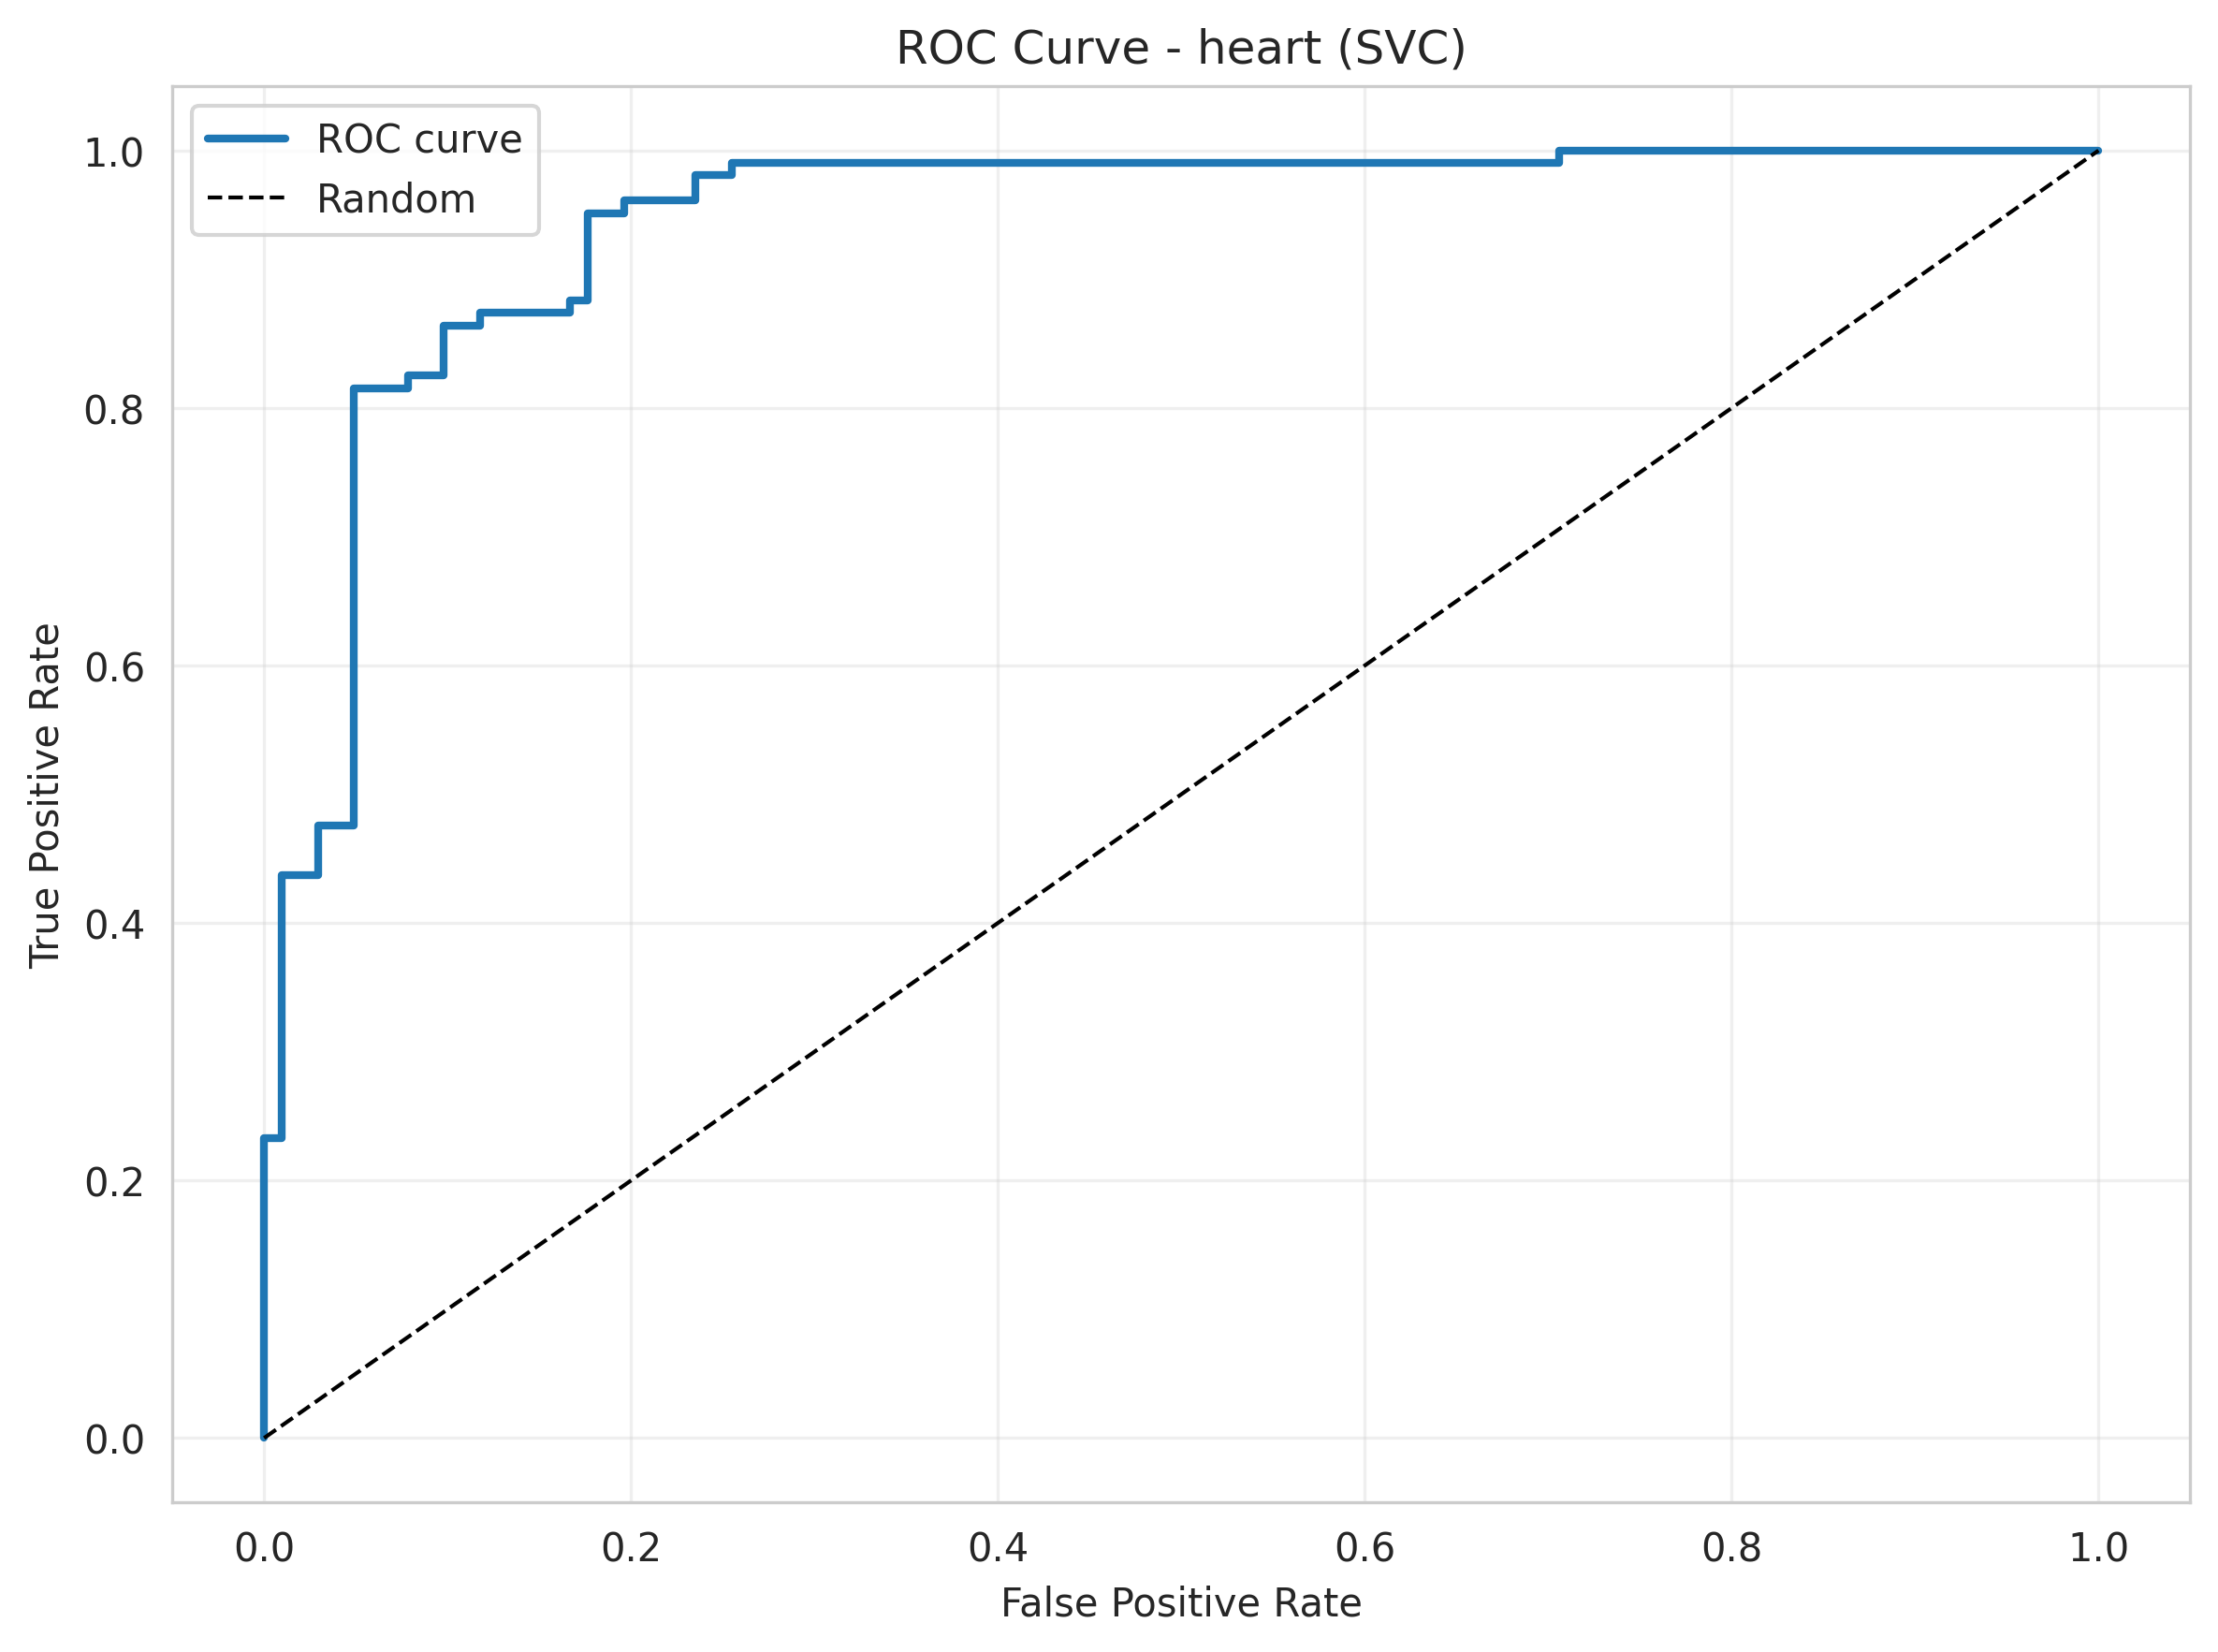
\includegraphics[width=0.7\textwidth]{images/roc_curve_heart_svc.png}
\caption{ROC-кривая — Heart Disease Dataset (SVC)}
\end{figure}

\subsection{Сравнение производительности моделей}

\begin{figure}[H]
\centering
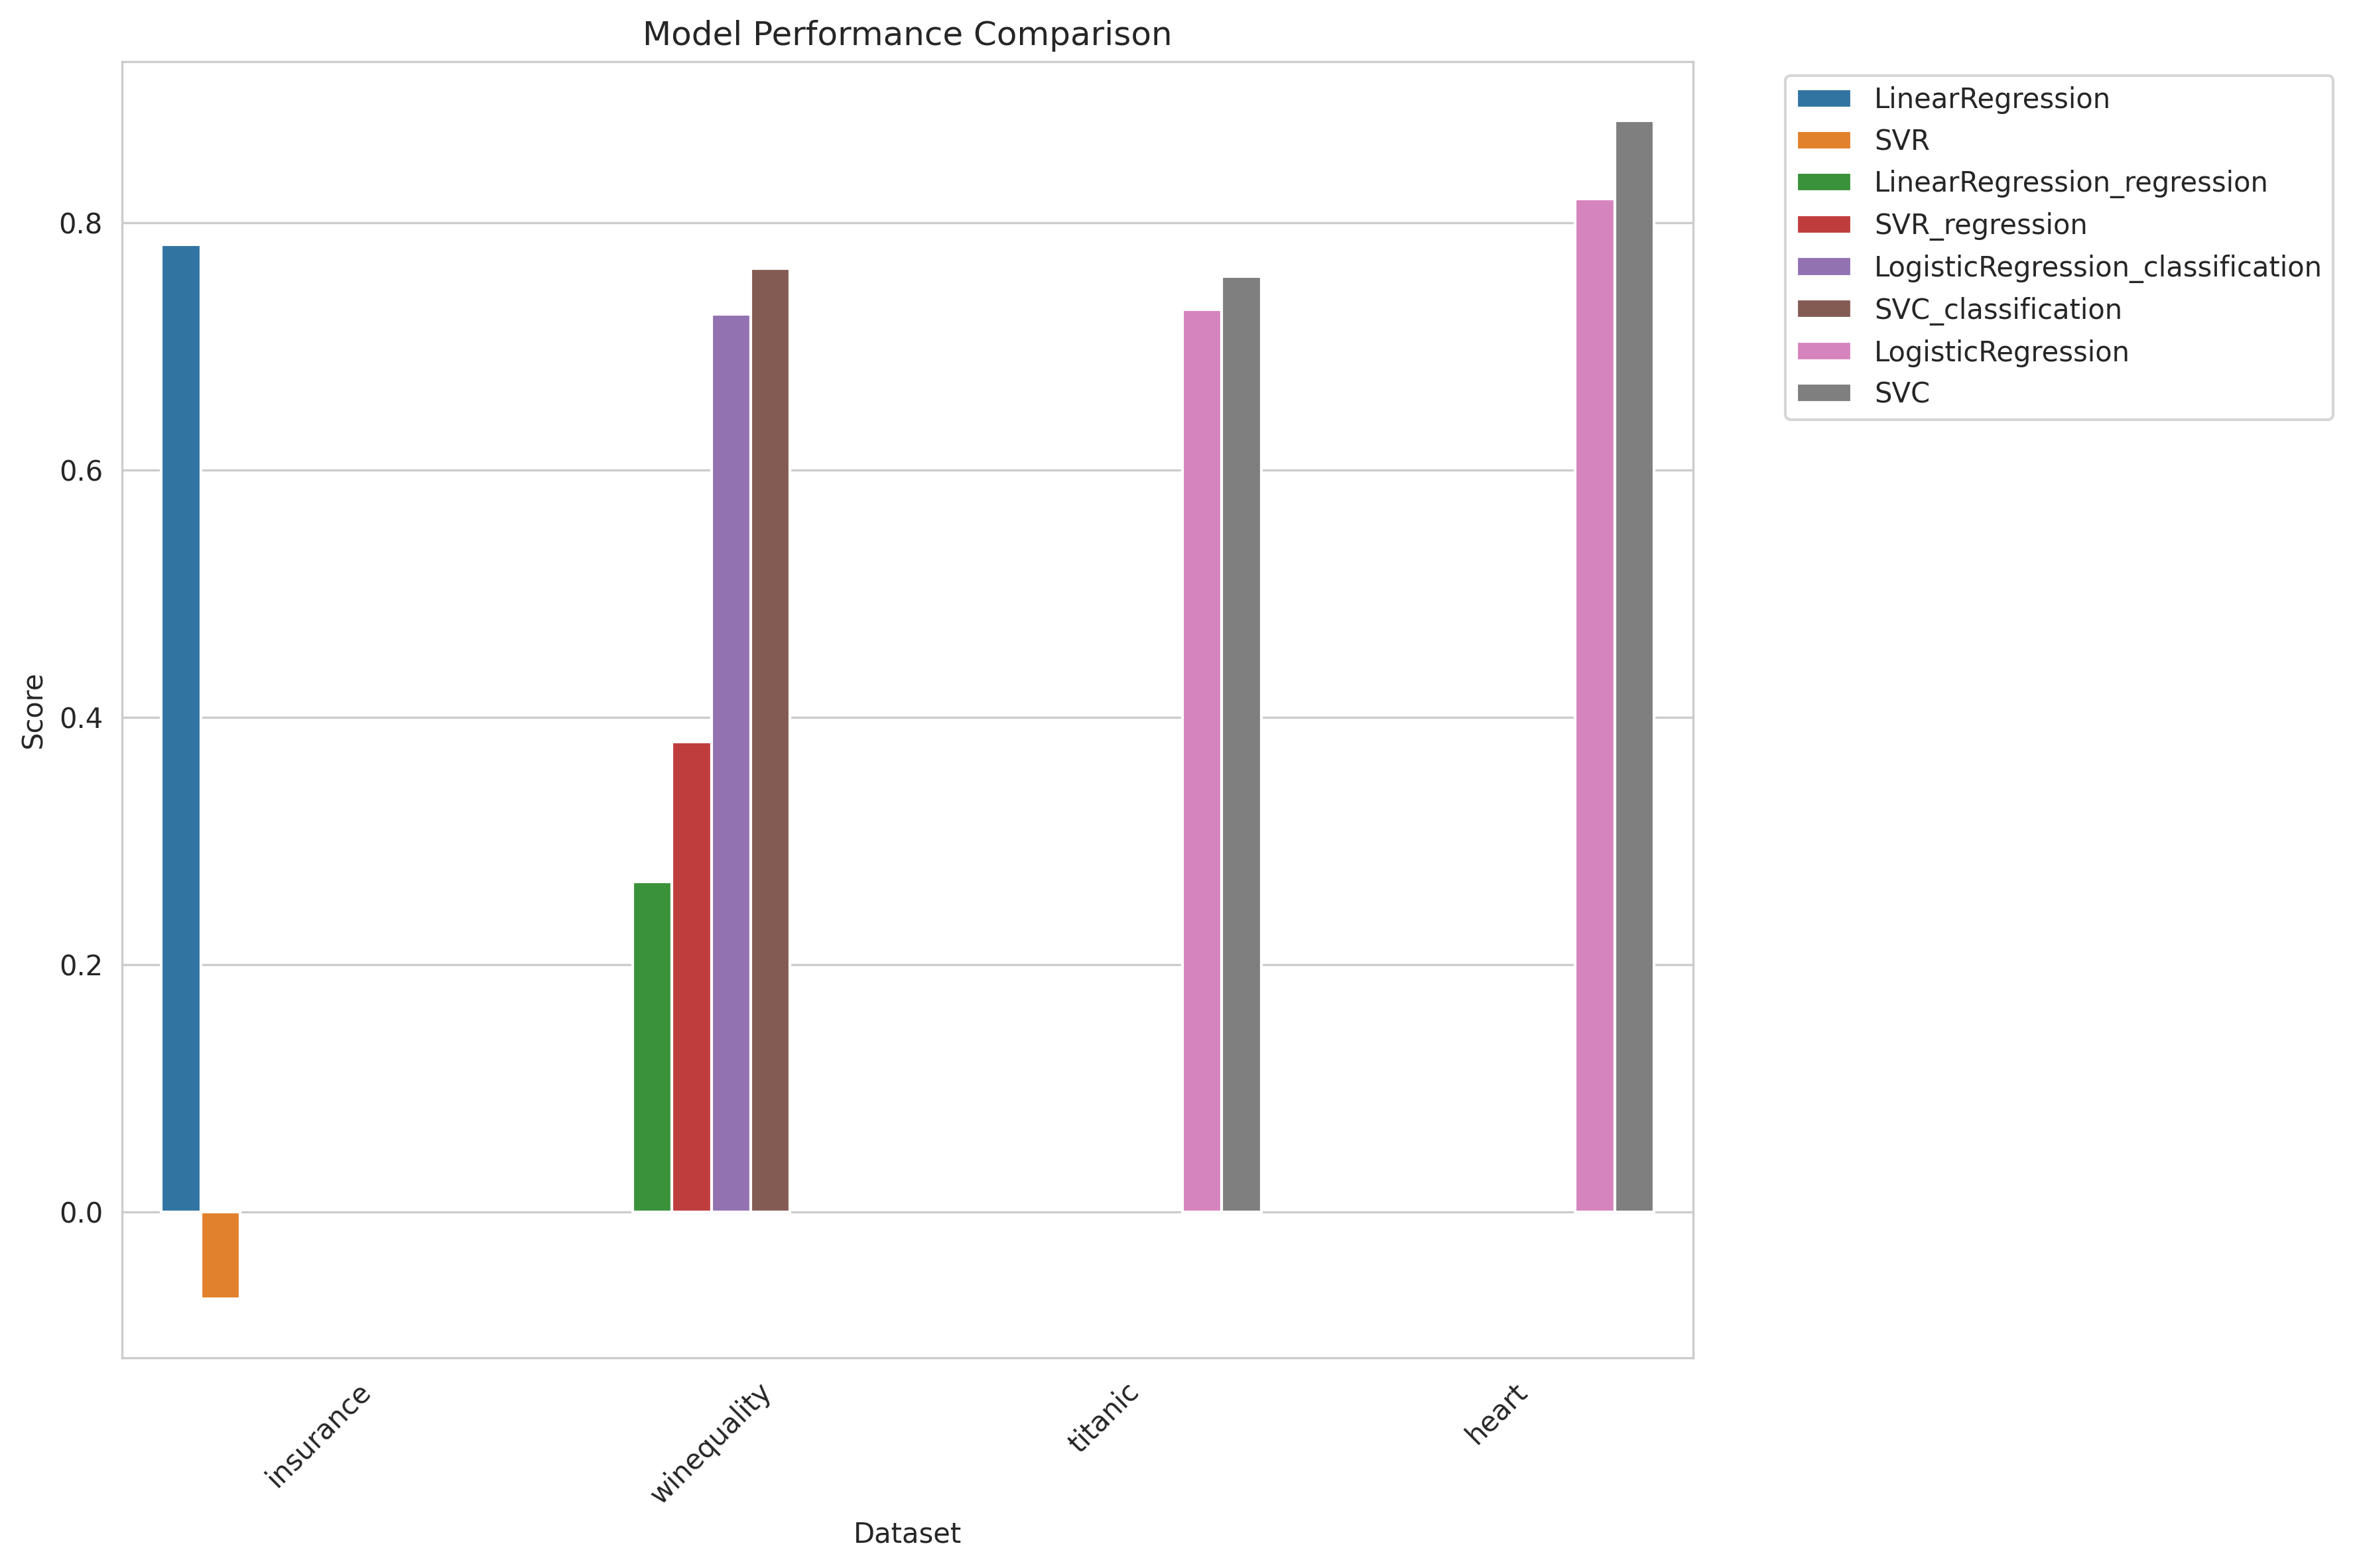
\includegraphics[width=0.9\textwidth]{images/model_comparison.png}
\caption{Сравнение моделей по основным метрикам качества}
\end{figure}

\section{Обсуждение результатов и выводы}

\subsection{Детальный анализ результатов по датасетам}

\subsubsection{Insurance Dataset — Регрессионная задача}

На датасете медицинской страховки тестировались методы регрессии:
\begin{itemize}
    \item Linear Regression: RMSE = 5810.028, R² = 0.783
    \item SVR: RMSE = 12891.136, R² = -0.070
\end{itemize}

\textbf{Анализ результатов:}
Линейная регрессия показала значительно лучшие результаты. R² = 0.783 означает, что модель объясняет около 78\% дисперсии в стоимости страховки. SVR с отрицательным R² работает хуже простого предсказания среднего значения.

\textbf{Возможные причины различий:}
\begin{enumerate}
    \item Линейный характер зависимости между признаками и стоимостью страховки
    \item Недостаточная настройка гиперпараметров SVR (C, gamma, epsilon)
    \item Относительно небольшой размер датасета для эффективной работы SVM
    \item Особенности предобработки данных, более подходящие для линейных методов
\end{enumerate}

\subsubsection{Wine Quality Dataset — Смешанная задача}

Для датасета качества вина проводились эксперименты как с регрессией, так и с классификацией:

\textbf{Регрессия (предсказание оценки качества):}
\begin{itemize}
    \item Linear Regression: RMSE = 0.736, R² = 0.267
    \item SVR: RMSE = 0.677, R² = 0.380
\end{itemize}

\textbf{Классификация (хорошее/плохое вино, порог ≥6):}
\begin{itemize}
    \item Logistic Regression: Accuracy = 0.726, F1 = 0.792, AUC = 0.781
    \item SVC: Accuracy = 0.763, F1 = 0.820, AUC = 0.822
\end{itemize}

\textbf{Анализ результатов:}
В отличие от датасета Insurance, здесь SVR превосходит линейную регрессию. Это указывает на наличие нелинейных зависимостей между химическими свойствами вина и его качеством. R² около 0.38 для SVR показывает умеренную предсказательную способность.

Для задачи классификации SVC также показал лучшие результаты, что подтверждает эффективность нелинейного разделения классов.

\subsubsection{Titanic Dataset — Классификация выживаемости}

\begin{itemize}
    \item Logistic Regression: Accuracy = 0.730, F1 = 0.792, AUC = 0.814
    \item SVC: Accuracy = 0.757, F1 = 0.816, AUC = 0.863
\end{itemize}

\textbf{Анализ результатов:}
SVC превосходит логистическую регрессию по всем метрикам. AUC = 0.863 указывает на хорошую способность модели различать выживших и погибших пассажиров. Это может быть связано со сложными взаимодействиями между признаками (возраст, класс билета, пол).

\subsubsection{Heart Disease Dataset — Медицинская диагностика}

\begin{itemize}
    \item Logistic Regression: Accuracy = 0.820, F1 = 0.833, AUC = 0.906
    \item SVC: Accuracy = 0.883, F1 = 0.891, AUC = 0.945
\end{itemize}

\textbf{Анализ результатов:}
Этот датасет показал наилучшие результаты среди всех задач классификации. AUC = 0.945 для SVC указывает на отличную диагностическую способность модели. Это может быть связано с:
\begin{enumerate}
    \item Хорошо подобранными медицинскими признаками
    \item Оптимальным размером выборки
    \item Четкими границами между классами в пространстве признаков
\end{enumerate}

\subsection{Сравнительный анализ методов}

\subsubsection{Линейная vs. Логистическая регрессия}
Оба метода показали стабильную работу на всех датасетах. Логистическая регрессия особенно эффективна как базовый метод для задач классификации, обеспечивая:
\begin{itemize}
    \item Интерпретируемость результатов
    \item Быстроту обучения
    \item Надежность предсказаний
\end{itemize}

\subsubsection{SVM vs. Линейные методы}
SVM показал превосходство в большинстве задач, особенно для классификации:
\begin{itemize}
    \item \textbf{Преимущества SVM:} способность работать с нелинейными зависимостями, устойчивость к выбросам, хорошая обобщающая способность
    \item \textbf{Недостатки SVM:} вычислительная сложность, необходимость настройки гиперпараметров, меньшая интерпретируемость
\end{itemize}

\subsection{Факторы, влияющие на производительность}

\subsubsection{Характеристики данных}
\begin{enumerate}
    \item \textbf{Размер выборки:} SVM лучше работает на средних и больших выборках
    \item \textbf{Размерность:} после One-Hot кодирования некоторые датасеты получили высокую размерность (Titanic — 462 признака)
    \item \textbf{Качество признаков:} медицинские данные (Heart Disease) показали лучшие результаты
    \item \textbf{Балансировка классов:} влияет на метрики классификации
\end{enumerate}

\subsubsection{Предобработка данных}
Качество предобработки критически важно:
\begin{itemize}
    \item Стандартизация особенно важна для SVM
    \item One-Hot кодирование может создавать разреженные матрицы
    \item Обработка пропущенных значений влияет на размер выборки
\end{itemize}

\subsection{Практические рекомендации}

\subsubsection{Выбор метода в зависимости от задачи}

\textbf{Для регрессионных задач:}
\begin{itemize}
    \item Начинать с линейной регрессии как базового метода
    \item Использовать SVR при подозрении на нелинейные зависимости
    \item Проводить тщательную настройку гиперпараметров SVR
\end{itemize}

\textbf{Для задач классификации:}
\begin{itemize}
    \item Логистическая регрессия — хороший базовый метод
    \item SVC рекомендуется для улучшения качества при наличии ресурсов
    \item Обязательная кросс-валидация для выбора гиперпараметров
\end{itemize}

\subsubsection{Вычислительные аспекты}
\begin{enumerate}
    \item \textbf{Время обучения:} Линейная/логистическая регрессия < SVM
    \item \textbf{Время предсказания:} Все методы показывают сопоставимую скорость
    \item \textbf{Память:} SVM требует больше памяти для хранения опорных векторов
\end{enumerate}

\subsection{Ограничения исследования}

\begin{enumerate}
    \item \textbf{Гиперпараметры:} Использовались значения по умолчанию, что могло негативно повлиять на производительность SVM
    \item \textbf{Кросс-валидация:} Не применялась, что снижает надежность оценок
    \item \textbf{Инженерия признаков:} Не проводилась специфическая для каждого датасета работа с признаками
    \item \textbf{Ансамблевые методы:} Не рассматривались, хотя могли бы показать лучшие результаты
\end{enumerate}

\subsection{Заключение}

Проведенное исследование показало, что выбор метода машинного обучения существенно зависит от характеристик данных и специфики задачи. SVM продемонстрировал превосходство в задачах классификации, особенно при наличии сложных нелинейных зависимостей. Линейные методы остаются эффективными для задач с линейными зависимостями и являются хорошим базовым выбором.

Для практического применения рекомендуется:
\begin{itemize}
    \item Начинать с простых методов (линейная/логистическая регрессия)
    \item Проводить тщательную предобработку данных
    \item Использовать кросс-валидацию для выбора гиперпараметров
    \item Рассматривать SVM для повышения качества при наличии ресурсов
    \item Учитывать специфику предметной области при интерпретации результатов
\end{itemize}

Данное исследование подтверждает важность эмпирического сравнения методов для каждой конкретной задачи, поскольку теоретические преимущества не всегда соответствуют практическим результатам.

\end{document}